\documentclass[12pt]{article}
\usepackage{blindtext}
\usepackage[utf8]{inputenc}
\usepackage{listings}
\usepackage{mathtools}
\usepackage{graphicx}
\usepackage{matlab-prettifier}
\usepackage{subcaption}
\usepackage[margin=1.3in]{geometry}
\addtolength{\topmargin}{-.5in}
\linespread{1}
\usepackage{setspace}
\usepackage{fancybox}
\usepackage{amsmath}% http://ctan.org/pkg/amsmath
\usepackage{array}
\usepackage{tabu}
\usepackage{bm}
\usepackage{float}
\usepackage{listings}             % Include the listings-package
\setlength{\parindent}{0pt}
\bibliographystyle{IEEEtran}
\captionsetup{justification=centering}

\lstset{language=Java,
basicstyle=\ttfamily\scriptsize,
keywordstyle=\color{javapurple}\bfseries,
stringstyle=\color{javared},
commentstyle=\color{javagreen},
morecomment=[s][\color{javadocblue}]{/**}{*/},
numbers=left,
numberstyle=\tiny\color{black},
stepnumber=2,
numbersep=10pt,
tabsize=4,
showspaces=false,
showstringspaces=false,
breaklines=true,
frame=single}

\definecolor{grey}{rgb}{0.9,0.9,0.9} % Color of the box surrounding the title - these values can be changed to give the box a different color

\definecolor{javared}{rgb}{0.6,0,0} % for strings
\definecolor{javagreen}{rgb}{0.25,0.5,0.35} % comments
\definecolor{javapurple}{rgb}{0.5,0,0.35} % keywords
\definecolor{javadocblue}{rgb}{0.25,0.35,0.75} % javadoc

\thispagestyle{empty}

\date{16 March 2017}

\begin{document}
\vspace*{6cm}
\colorbox{white}{
	\parbox[t]{1.0\linewidth}{
		\centering \fontsize{50pt}{80pt}\selectfont % The first argument for fontsize is the font size of the text and the second is the line spacing - you may need to play with these for your particular title
		\vspace*{0.7cm} % Space between the start of the title and the top of the grey box

		{401I - Final Year Project} \break
		\vspace*{0.7cm}
		Final Report
		\break
		Voice Recognition RPG
		\break
		Baron Khan (bak14)
		\vspace*{0.7cm} % Space between the end of the title and the bottom of the grey box
	}
}
\vfill % Space between the title box and author information




\newpage
\thispagestyle{empty}
\tableofcontents
\newpage
\setcounter{page}{1}
\section{Abstract}

\textbf{When adding voice commands to a video game, a developer may find themselves hard-coding text strings for phrases that a player can say, and mapping them to intents within the game. It becomes more work to include varying versions of the same intent as the developer would have to include every permutation of the phrase (for which there could be infinitely many).
\\
\\
This project presents a text-based role-playing game (RPG) on Android which allows the player to issue actions within the game using their voice. The game uses a new voice recognition system that aims to make it easier for the developer to add voice commands without hard-coding the phrases.
\\
\\
We explore and evaluate various methods for improving the voice recognition system with the aim of decreasing the developer workload. These include using semantic similarity methods, adaptive and user-controlled learning mechanisms, and various other NLP techniques. We also explore various other ways of making the development of the role-playing game easier (such as automated room generation).}

\newpage

\section{Introduction}
In recent years, video games have explored various forms of input that diverge from the traditional control schemes of a keyboard and mouse, or an analogue stick and buttons on a controller. Touch-screen controls and motion controls have had varying degrees of success over the years, and provide new forms of interactions with games. A recent form of input used in video games has been voice controls; a user utters a sentence or phrase and this would execute an action or intent within the game.
\\
\\
Voice recognition and control schemes have been used in various ways in the medium, whether in tandem with traditional control schemes, or as the only form of input. Most games which feature a voice control scheme are typically programmed to work with a specific set of keywords or phrases, hard-coded by the developer. This is usually the case with games where the voice control interface is entirely optional to user, as it requires little to no input from the programmer; if the speech processing is handled by a separate library, the developer just has to map a text string (e.g. "open the door") to the function that executes the intent (e.g. the function that opens a nearby door in the game).
\\
\\
It becomes increasingly difficult for the developer to add more phrases that can be accepted in the game and map to the same intent (e.g. "push the door open") as they would have to hard-code each possible input that the user could possibly say: having too few phrases would mean that the user could become frustrated when their preferred way of stating an intent is not accepted by the game, while adding too many acceptable phrases would increase development time.
\\
\\
Natural Language Processing (NLP, also referred to as Natural Language Understanding) has been used to improve inference of what users were trying to say, and to extract meaning from the user's phrases and sentences. For instance, if the user says, "push the door open", NLP can be used to infer that the user's intent is to open a door. Using NLP, several user phrases can be mapped to the same intent without having to hard-code each possible phrase.
\\
\\
NLP is already used to improve voice recognition in popular personal assistants such as Siri, but these systems offload the NLP workload to the server to reduce the amount of local processing required, as NLP requires a sizeable amount of machine learning and pattern recognition \cite{RefWorks:21}. Most video games do not require an internet connection to play, and therefore can be played anywhere, so it may not be possible to use these cloud services for adding voice recognition to games.
\\
\\
The goal of this project is to apply NLP to a voice control scheme used within a role-playing game (RPG), in order to reduce the amount of work required by a developer to add a flexible voice control interface, and to give more freedom of expression to the player while they play the game.
\\
\\
Role-playing games are a genre of video games that involve the player controlling a character in a world featuring exploration and/or battle mechanics, along with a progression system, where the character gains new abilities or items as the game progresses. These include turn-based games such as Pokemon and Final Fantasy, or more action-based games such as Dark Souls or Skyrim. In these games, the player possesses several items that they acquire during the game, and accesses them by navigating menus.
\\
\\
If the player has many different items, they may need to spend a lot of time searching the menus for a specific item, which can be quite tedious. It can also become quite repetitive if the user is constantly only pushing the "Attack" button over and over again with no variation in the attack used. Using voice recognition and NLP, a player could just simply say a phrase such as, "use a potion" or, "attack with axe", and the item will be used without having the player navigate several menu screens.
\\
\\
Another motivation for this project is to explore how voice controls can allow games to become more accessible to people with certain disabilities that prevent them from using traditional controllers or a keyboard and mouse. Very few popular games support voice recognition as a form of control, whether it is consoles, PC or mobile.
\\
\\
A text-based RPG will be created that will use a flexible voice control interface. It will feature a simple exploration mechanic, with the user manipulating objects and environments using voice commands, and a simple battle mechanic. These will be designed to fully demonstrate the power of the voice-control system to make the game easier to play, as opposed to using traditional mouse clicks and button presses. The target platform will be Android to allow for hands-free voice control input.
\\
\\
Note that this project is not concerned with the real time digital processing required to convert speech to text; it is assumed that the speech from the microphone is already converted to a text string using an existing tool such as Google's Speech-to-Text API. The focus is on the integration and usability of voice control schemes.
\\
\\
The proposed design for the RPG and system aims to achieve the following goals:
\begin{itemize}
\item Allow a developer to add voice recognition to their game with little effort.
\item Create a simple natural language processing system that can work offline.
\item Explore NLP usages in RPGs (for text generation, item descriptions, etc).
\end{itemize}

\newpage
\section{Background}

\subsection{Voice Recognition in Games}
Below is a list of notable recent games that have incorporated voice control functionality as a major component of the interaction experience.
\subsubsection{In Verbis Virtus}
In Verbis Virtus \cite{RefWorks:22} is an independent 3D fantasy adventure game developed by Indomitus Games for Windows. It requires the player to solve puzzles in a 3D environment and battle enemies using magic.
\\
\\
When a microphone is connected, the player is able to cast spells using their voice by saying specific phrases defined by the game. For example, to cast a spell that produces a floating light source to brighten a room, a user must say, "let there be light", or if the user wishes to shoot an energy beam from their hand, they must say, "Beam of Light", and so. These phrases appear to be hard-coded into the game.
\\
\\
There are several limitations with this implementation of voice control. Firstly, since the phrases are hard-coded, there is no lenience in variations of the phrases, e.g. "create a light" or "Laser of Light", etc. This can seem mundane and no different to a user pressing the same button repeatedly to cast a spell.
\\
\\
Another limitation is that the user is still required to use a keyboard and mouse to perform other actions in the game, such as moving around, looking around, and navigating menus and message boxes. The voice control interface cannot be used to perform these actions. The voice control interface itself does not seem integral to the experience, as the user could just simply press a key that performs the spell instead of saying the same phrase over and over again.
\\
\\
This voice recognition interface could be improved by allowing the player to perform any action within the game using their voice, as well as allowing for more variation in what the user can say for each action.

\subsubsection{Skyrim Kinect}
The Elders Scrolls V: Skyrim is first-person action role-playing game developed by Bethesda \cite{RefWorks:23}. The Xbox 360 version of the game supports the Microsoft Kinect peripheral which allows the player to execute voice commands \cite{RefWorks:24}. The user can use over 200 hundred pre-configured voice commands, and these can be used simultaneously with the traditional control scheme.
\\
\\
There are voice commands available that allow the user to navigate the game's menu screens. For instance, the player would say, "quick items" to open their inventory menu. Afterwards, the user can open menus for specific categories of items such as "potions", "books", etc. However, it doesn't seem to be possible to actually use any of the items selected with only a voice command from the menu; this is only possible if you assign the item to a 'hotkey' (e.g. by saying, "assign health potion" once you have highlighted a potion item), and then saying "equip health potion" during the game. See the Appendix \ref{appendix:skyrim} for a full list of available voice commands.
\begin{center}
\begin{figure}[H]
  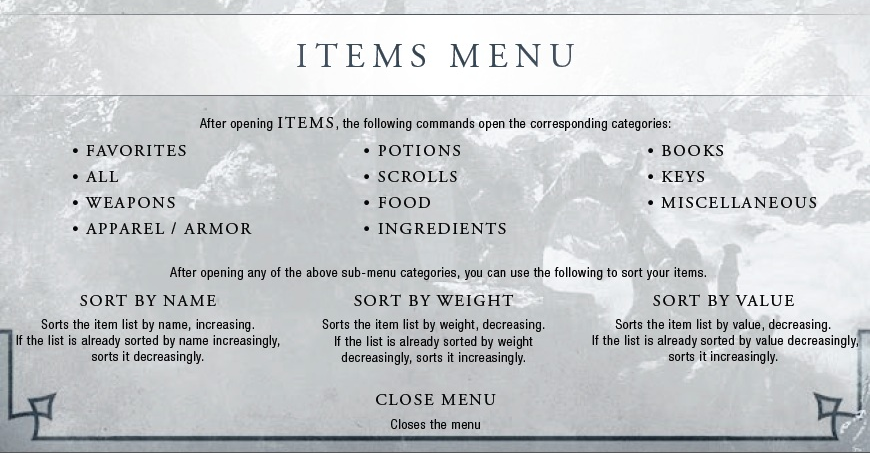
\includegraphics[width=\textwidth]{skyrim-item-commands.png}
  \caption{Voice commands that are available within the items menu in Skyrim.}
\end{figure}
\end{center}
This system, despite being optional to the player, helps to reduce the time spent searching through the menu screens. However, it appears that this system also hard-codes the phrases that can be said by the player with no flexibility.

\subsubsection{Star Trek Bridge Crew}

Star Trek Bridge Crew is a virtual reality game developed by Ubisoft. This game allows the player to issue voice commands to AI crew members on a spaceship \cite{RefWorks:29}. In order to develop a more interactive and realistic experience, the development team used IBM Watson's interactive speech capabilities. This API allows commands to be delivered in a variety of ways, as the speech is parsed for its meaning using Watson's Conversation service. For example, a player could say, "show me the ship's status report" or they could say something drastically different such as "damage report" to execute the same command \cite{RefWorks:25}. This gives the user more freedom in how they convey their request to the AI, giving the player a "new level of sense of presence" \cite{RefWorks:26}. IBM's Watson API is described in more detail later in this section.
\\
\\
The voice recognition design used in this game is similar to the proposed design outlined in this report. The user's intent should be extracted from the phrase that they speak, so similar phrases should map to the same intent. Unfortunately, Watson's API is a paid cloud service; so the game requires a constant internet connection to play.

\subsubsection{Classic Zork on Alexa}

Zork is a trilogy of classic text-based role-playing games that support a free-form style of input. The player is provided with an input scenario (e.g. "You are standing in an open field west of a white house, with a boarded front door. There is a small mailbox here."), and then types commands that they want to execute (e.g. "open mailbox" or "attack troll with sword") \cite{RefWorks:35}. The exploration part of the proposed game in this report will be loosely based off Zork's exploration mechanics of interacting with objects in the surroundings.
\\
\\
These commands could be delivered using a speech-to-text interface to add voice control to Zork. A group of developers created a port of Zork running on Amazon's Alexa Skills Kit \cite{RefWorks:37}. This allows the player to deliver commands using their voice as if they were typing the phrases into a terminal. However, this implementation still suffers from the limitations of Zork's free-form input.

\subsection{Limitations of Zork}

The exploration mechanics of the proposed design in this report will be based on Zork's general gameplay of interacting with objects in the environment to solve puzzles, and the limitations of Zork's free-form input are discussed here.
\\
\\
Zork supports a number of text commands, which usually take the form of a verb-noun structure, such as "use $<$noun$>$" or "take $<$noun$>$", but it also supports some more sophisticated commands with complex structures, such as "give all but the pencil to the nymph" or "drop all except the dart gun" \cite{RefWorks:36}.
\\
\\
Zork's free-form input still has some limitations. For example, it still cannot accept all variations of specific intents. For instance, below is a list of accepted and rejected commands if the user wishes to open a mailbox in front of them:
\begin{itemize}
	\item "open mailbox" - Accepted
	\item "open the small mailbox" - Accepted
	\item "can i open the mailbox" - Rejected
	\item "check the mailbox" - Rejected
	\item "find out what's in the mailbox" - Rejected
\end{itemize}
Below is a list of results for closing the mailbox:
\begin{itemize}
	\item "close mailbox" - Accepted
	\item "shut mailbox" - Rejected
	\item "closing mailbox" - Rejected
	\item "close the red mailbox" - Rejected
\end{itemize}
Clearly the rejected text commands could be valid phrases that express an intent to open some sort of mailbox. Zork has a pre-defined list of verbs and sentence structures that it can accept, and sticks to those without much flexibility.
\\
\\
Since most of the supported commands take the form of a verb-noun structure, this could be used in the proposed design as the general structure of commands expected by the user.

\subsection{Voice Recognition Implementations}

There are many tools and services available that allow developers and users to add voice recognition to video games, with some discussed below:

\subsubsection{Tazti - Speech Recognition for PC Games}

Tazti is a keyboard mapping tool available to players to be used with any type of PC game that uses the keyboard \cite{RefWorks:28}. The user sets up a profile for each game separately by mapping speech commands to one or more keys. For instance, the user could say "fire" or "shoot fire" and this would map to the keystrokes required to cast a fire spell.
\\
\\
While this tool is not directly integrated into games by the developer, it has the advantage of being able to work with almost any PC game that uses a keyboard, such as role-playing games, first-person shooter games, and even platforming games. However, the voice commands are limited to being hard-coded, so there is no way of varying the speech commands slightly, even if the meaning is the same. It is also not freely available and requires a license to be purchased.

\subsubsection{PocketSphinx for Unreal Engine 4}

\textit{Sphinx-UE4} is a speech recognition plugin for the Unreal Engine 4 game engine \cite{RefWorks:104}, based on the PocketSphinx library which provides offline speech-to-text \cite{RefWorks:105}. The plugin allows the developer to specify keywords and the commands that they map to (e.g. "turn right", "enable sprint", "kick the ball", etc).
\\
\\
The plugin also supports grammar files. A grammar contains the grammatical structure that an accepted input can take, such as, $<digit> <operation> <digit>$. This will accept input such as, "three add five", "six minus four", "two times twelve", and so on.

\subsubsection{Houndify}

Houndify is a paid cloud service developed by SoundHound that allows developers to add voice recognition and control to any application they wish \cite{RefWorks:30}. The API takes as input either a text string or audio samples and returns a JSON string containing the response to the input. This response can range from anything: from home automation control, to weather updates, and more. The response would be in the form of an intent - a single word representing the action to be executed. For example, any attacking phrase would map to an intent called, "ATTACK".
\\
\\
As well as having built-in voice commands already for specific domains (such as all weather commands or sports update commands), Houndify also supports the creation of custom voice commands by the developer. To create a custom command, the expression to be said by the user is specified using a syntax similar to regular expressions, but instead specifies the general phrase structure (and with very different syntax), and is mapped to an intent \cite{RefWorks:33}.
\\
\\
Below is an example of a possible expression for attacking a troll:
\begin{center}
"attack" . "troll"
\end{center}
Here, the player would have to say, "attack troll" to execute the intent. This can be expanded to have more variation in how the user can say this command:
\begin{center}
("attack" $\vert$ "hit") . ["the"] . "troll"
\end{center}
Here, the player can say phrases such as, "attack the troll" or "hit troll". The expression can be further expanded. However, the expression will eventually become long and confusing:
\begin{center}
("attack" $\vert$ "hit" $\vert$ "damage") . ["the"] . ["big" $\vert$ "large"] . "troll" . [("with" $\vert$ "using") . ["a"] . ("sword" $\vert$ "hammer" $\vert$ "axe")]
\end{center}
Even though this expression allows for more variation in what the user can say, it still doesn't cover all the possible variations of specifying an attack, and this long expression is only for one intent; many more expressions would have to be written for other intents, and this can become tedious for the developer.
\\
\\
While this API would be useful for building a personal assistant similar to Apple's Siri or Amazon's Alexa, it does not seem feasible for this project due to the time required to create a flexible voice recognition scheme. This is also a paid service, so users are charged for each query they make.

\subsubsection{Watson Conversation Engine}

IBM's Watson API features a Conversation service that allows developers to build voice recognition interfaces that understand natural language input \cite{RefWorks:27}. The developer defines the training data to be used by the API (in order to train a natural language classifier) using 'intents' and 'entities' \cite{RefWorks:31}.
\\
\\
'Intents' are the goals that a user will have as they interact with the application. For example, in a voice-controlled car, an intent could be 'wipers\textunderscore on', in order to activate the windscreen wipers. This intent would be paired with example utterances in the form of text strings, such as "turn on the wipers", "switch on the windscreen wipers", and so on. The more examples given, the more accurate the trained model will be.
\begin{center}
\begin{figure}[H]
  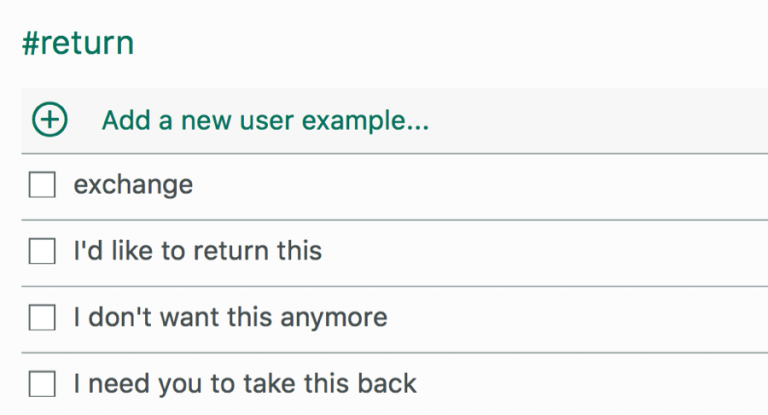
\includegraphics[width=\textwidth]{intent-return.png}
  \caption{An example of an intent to return something, along with examples of phrases for the intent. Image re-used from an IBM blog post \cite{RefWorks:34}.}
\end{figure}
\end{center}
'Entities' are classes of objects that help to provide context to intents. For example, in the above example, it is not clear whether the user is referring to the wipers on the front of the car or the wipers on the back of the car (the API will assume the front by default). If the entity is included in the phrase spoken by the user, then the context of the intent becomes clear.
\begin{center}
\begin{figure}[H]
  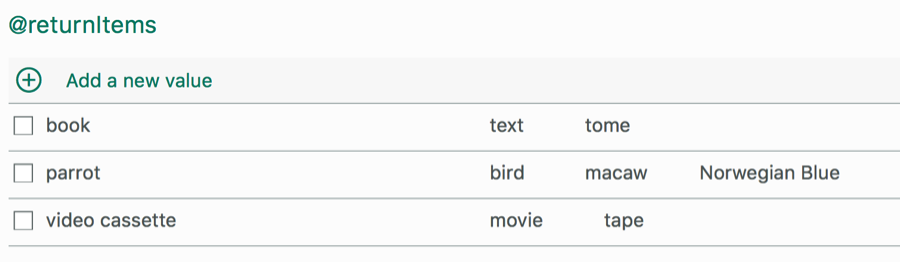
\includegraphics[width=\textwidth]{returnitems.png}
  \caption{An example of entities for items that can be returned. Entities that have been grouped together (usually synonyms) are placed on the same row \cite{RefWorks:34}.}
\end{figure}
\end{center}
Once the classifier is trained, it will be able to use the examples of intents provided to classify whether new examples of phrases have the same meaning as those. For example, if the user says, "activate the windscreen wipers at the front of the car", the classifier will return the 'wipers\textunderscore on' intent, even though this input is very different in structure to the examples provided above. A demo is available to test this \cite{RefWorks:32}.
\\
\\
This API is very flexible and matches the first objective of this project; only a few example of possible inputs need to be provided for each intent, and then the classifier can infer whether any new input strings will match the same intent. Unfortunately, despite being a very powerful system, this still remains a paid cloud service, so users are charged per API call. It also requires a lot of processing power (which is offloaded to a cloud server) for the many machine learning algorithms being used here. However, a simpler system may possibly be implemented that uses a similar concept to the intents and entities framework, and the proposed design in this report uses a similar concept that runs locally.
\\
\\
According to a research paper by McCord, Murdok and Boguraev on \textit{Deep Parsing in Watson} RRR, the engine consists of two deep parsing components: an English Slot Grammar (ESG) parser and a a predicate-argument structure (PAS) builder. These allow Watson to produce parse trees of a sentence and extract pattern-based relations from it, such as question decomposition, hypothesis generation, and evidence scoring.
\\
\\
There is a similar API called DialogFlow \cite{RefWorks:106}, which works very similarly to IMB's Watson Conversation engine. However, it suffers from the same issues as above (e.g. cloud-based, pay-per-request, etc).

\subsection{Natural Language Processing}

Natural Language Processing (NLP) forms a major component of this project. This will give the developer the ability to take an arbitrary string of text and infer its meaning, and map it to an intent. Below are some explanations on NLP concepts related to this project.

\subsubsection{Stages of Natural Language Processing}

\begin{center}
\begin{figure}[H]
  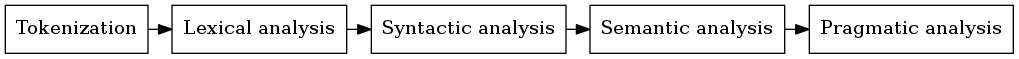
\includegraphics[width=\textwidth]{nlp-stages.png}
  \caption{The general stages of processing a text string for its meaning using NLP.}
\end{figure}
\end{center}

NLP can be broken down into six stages \cite{RefWorks:38}. The first stage is the tokenisation, where a raw text string is broken down into words (usually separated by spaces).
\\
\\
The second stage is the lexical analysis, where the output of the tokenisation process is improved upon by looking at words that can be taken apart even further (or rejoined if needed) to uncover more information. These include words such as: clictic contractions (e.g. "what're" would tokenise to "what" and "are",. while "we're" would break down to "we" and "are"); removing end-of-line hyphens that split whole words into parts when using a justification alignment; and abbreviations (e.g. Dr., U.S.A., etc.) \cite{RefWorks:39}.
\\
\\
The third stage is syntactic parsing, where the grammatical structure of the sentence is determined. This is usually achieved by generating a syntax tree of each sentence, where each word is broken down into a terminal from a given grammar (e.g. verbs, nouns, adjectives, determiners, etc.) \cite{RefWorks:40}.

\begin{center}
\begin{figure}[H]
\begin{center}
  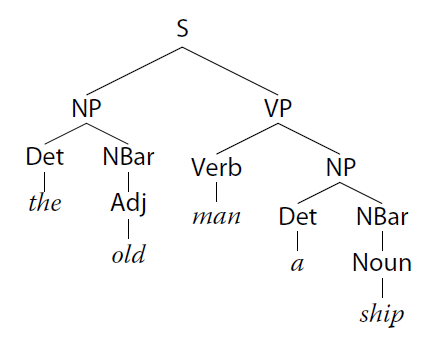
\includegraphics[scale=1]{syntax-tree.png}
  \caption{An example of a syntax tree for the sentence. "the old man a ship". Diagram taken from the Handbook of Natural Language Processing  \cite{RefWorks:40}.}
  \end{center}
\end{figure}
\end{center}

In the example above for the sentence, "the old man a ship", the word, "man" could be mistaken to be a noun, but in this case, the sentence is implying that the elderly control a ship, and therefore, "man" is actually a verb here. This meaning can be more easily inferred when the sentence is broken down using a syntax tree, as above.
\\
\\
The final two stages are very similar and is difficult to separate them into separate stages. Both stages involve determining the meaning of the sentence. The fourth stage is often concerned with semantic analysis, whereas the last stage is more concerned with discourse analysis \cite{RefWorks:39}.

\subsubsection{Part-of-Speech Tagging}

A technique often used in NLP is to try to label each word with its correct part of speech, known as part-of-speech (POS) tagging. POS-tagging systems generally use a tagset containing POS tags to assign a tag to each word. The most popular tagset is the Penn Treebank tagset. This consists of 48 tags, of which 12 are for punctuation and other symbols \cite{RefWorks:41}. See the Appendix \ref{appendix:penn} for the full Penn Treebank tagset.
\\
\\
There are two main challenges regarding POS tagging. The first challenge is that words can sometime be ambiguous. That is, the word can be assigned a number of possible POS tags depending on its context. For instance, the word, "can" can either be a verb ("I can..."), a noun ("a can of tuna"), or another verb with a completely different meaning to the previous ("can that noise!") \cite{RefWorks:43}. The many meanings that are attributed to a word are known as its word senses.
\\
\\
The second challenge are words that are unknown to the tagger and cannot be tagged. A default tag is required for words which are unknown, but that could interfere with the rest of the POS-tagging process \cite{RefWorks:41}.
\\
\\
The proposed design for this project will use an open-source POS tagger in order to identify specific words in the player's input, namely verbs and nouns.

\subsubsection{Slot Filling}

According to the authors of \textit{Speech and Language Processing} \cite{RefWorks:107}, three tasks need to be done to understand a user's utterance to a chatbot. The first is \textit{domain classification}, to determine the topic that the user is talking about (e.g. weather, sport, etc), although this is unnecessary for single-domain applications such as the environment of a video game. The second task is \textit{intent determination} to determine the goal of the user, and finally, the last task is to do \textit{slot filling}.
\\
\\
Slot filling involves determining the specific details of an intent by defining a grammar that the intent must adhere to. An example for arithmetic operations would be, $<DIGIT1>$ $<OPERATION>$ $<DIGIT2>$. The input would be parsed by a context-free grammar parsing algorithm to extract each bit of information in order to fill each slot in the grammar.
\\
\\
A disadvantage to slot-filling using context-free grammar parsing is that not all valid expressions for an intent would match with the slots. A solution to this would be to define multiple grammars for different structures of inputs.

\begin{center}
\begin{figure}[H]
\begin{center}
  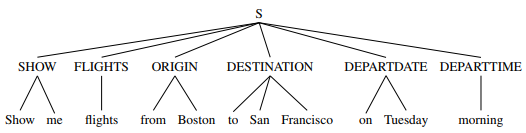
\includegraphics[scale=1]{slot-filling.png}
  \caption{An example of a slot-filling grammar for flights, using slot names as the internal parse tree nodes. Diagram taken from Chapter 29 of the book, \textit{Speech and Language Processing} \cite{RefWorks:107}.}
  \end{center}
\end{figure}
\end{center}


\subsubsection{Synonyms and Hypernyms}

Synonyms are words or phrases which have a similar meaning to another word  \cite{RefWorks:44}. For example, the word "dog" has seven word senses (different meanings), and for one of the word senses with a meaning of, "a member of the genus Canis", the synonyms would be, "domestic dog" and "Canis familiris" \cite{RefWorks:45}.
\\
\\
A hypernym, on the other hand, is a word or phrase which generalises words for which it is a hypernym of. For instance, the word, "instrument" is a hypernym of "guitar", because a guitar is a type of instrument. Similarly, the word "animal" is a hypernym of "cat" (or, at least, the sense which refers to the domestic animal, as "cat" can have several usages).
\\
\\
The synonyms and hypernyms of words and phrases can be represented as a hyper-tree structure, where the parent nodes are hypernyms of the child nodes, while each sibling node would represent a different word sense for a word, with each sibling containing the synonyms for that sense. Note that a hyponym is the inverse relationship between a word and its hypernyms.

\begin{center}
\begin{figure}[H]
\begin{center}
  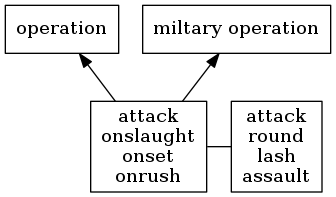
\includegraphics[scale=1]{hypernym-tree.png}
  \caption{A partial hypernym tree showing the synonyms and hypernyms for one of the senses of the noun, "attack". The "attack" verb sense (right) is a sibling node.}
  \end{center}
\end{figure}
\end{center}

Synonyms and hypernyms could be used to determine the semantic similarity between words and infer whether they match a certain intent of the user.

\subsubsection{Semantic Similarity}

There are many ways of calculating the semantic similarity between two words or phrases. Many of these methods use the synonyms and hypernym trees of the words to infer similarity, and assign a 'similarity score' to them. This score could be used to determine whether, for instance, a verb has semantic similarities to one of the intents in a game, and therefore can be mapped to that intent.
\\
\\
The following are some examples of measures for semantic similarity \cite{RefWorks:46}. The first is the Wu and Palmer (WUP) measure, which takes the depth in the hypernym tree of the Least Common Subsummer (LCS) (that is, the most general hypernym that both words have in common) and compares it with the sum of the depths of each word. The formula for the similarity of words $w_1$ and $w_2$ is as follows:

$$sim_{wup} = \frac{2*depth(LCS(w_1,w_2))}{depth(w_1)+depth(w_2)}$$

For example, the WUP score for the semantic similarity between "juice" and "water" is calculated as follows \cite{RefWorks:49}:

\begin{lstlisting}[frame=single]
T1 = HypernymTree( juice ) =
    [Sense #1] *ROOT* < entity < physical_entity < matter
    	< substance < food < foodstuff < juice

T2 = HypernymTree( water ) =
    [Sense #3] *ROOT* < entity < physical_entity < matter
    	< substance < food < water

Lowest Common Subsumer(s) = argmax(depth(subsumer(T1,T2)))
    = { subsumer(T1[1], T2[3]) } = { food }

DepthLCS = depth( food ) = 6
Depth1 = min(depth( {tree in T1 | tree contains LCS } )) = 8
Depth2 = min(depth( {tree in T2 | tree contains LCS } )) = 7
Score = 2 * DepthLCS / ( Depth1 + Depth2 ) = 2 * 6 / (8 + 7)
Score = 0.8
\end{lstlisting}

The WUP score of 0.8 out of 1.0 indicates that juice and water are semantically very similar \cite{RefWorks:47}, whereas the words "breathing" and "fire" only have a WUP score of 0.47, suggesting they are not semantically similar.
\\
\\
Another measure of semantic similarity is Leacock and Chodorow's method, which relies on the shortest distance between the two words in the hypernym tree, divided by the maximum depth of the whole tree; the shorter the distance, the more similar the words are \cite{RefWorks:46}. There are many more different measures and it is possible to combine them to produce an overall score for semantic similarity.

\subsubsection{Generating Sentences}

One feature for the proposed design of the RPG is to be able to generate text-based descriptions of the current situation that the player is in based on objects around them. For instance, a description could be, "You are in a room lit by a candle on a table. There is a piece of broken glass on the floor and a door in front of you." One could hard-code this sentence for each room the player visits, but if there are a lot of rooms in the game, this could become time-consuming. We would like to generate a sentence of the current situation based on sparse pieces of information (such as the items in the room, plus their locations, in a vector representation). This is the opposite of the intent inference described above, where the meaning of a sentence/phrase is extracted; we would like to be able to go in the opposite direction.
\\
\\
This is a relatively new field in NLP as it is particularly difficult. One method of sentence generation is suggested by Iyyer et al \cite{RefWorks:55}, where recursive autoencoders (a type of neural network) are used to generate a decomposition model of the sentence that can be used to reconstruct the sentence again. However, they found that proper nouns were not reconstructed correctly, and the model would need to be built in the first place to reconstruct the sentence.
\\
\\
Another group of researchers proposed a method of sentence generation which involves taking a sum of word embedding vectors and modelling it as a mixed integer programming problem \cite{RefWorks:54}. However, this also requires the original sentence to be de-constructed in the first place in order to know what the vector should contain.
\\
\\
One possible solution would be to only hard-code the general sentence structure of the description of rooms, and then insert the appropriate adjectives and nouns of the items, which is given as input in the form of a vector of strings.

\subsection{WordNet}

Princeton University created a large lexical database for the English language \cite{RefWorks:20}. Words are grouped into synonyms (known as synsets, or \textit{synonym sets}), and are connected to their respective hypernyms (more general words) and hyponyms (more specific words), creating the large hypernym tree mentioned previously. The database is open-source and is used extensively in this project, using various APIs that interact with the WordNet database (which will be initially downloaded by the game for offline use).

\subsection{Object Properties}

One issue to note is when a user attempts to specify an item based on a description of it (e.g. the user says, "attack the enemy with a sharp object"); we would like to be able to select a item that matches the description (e.g. a sword is sharp, so use that if the user possesses one). One approach to this is to assign to the items a set of properties such as whether it is sharp or blunt, whether it can be thrown, and so on.
\\
\\
A similar technique was used by the developers of Scribblenauts for the Nintendo DS. Using the company's ObjectNaut engine, the game utilises a large database of a hierarchy of objects \cite{RefWorks:48}. This allows them to design sprites for different objects (such as a cyborg, robot or android), but they have the same interaction properties. However, it still required the developers to go through encyclopaedias word-by-word. Using the semantic similarity scoring mechanism, this would not need to be done, as we can infer if two objects would have the same properties instead of hard-coding each one.
\\
\\
By assigning items different properties, we don't have to code the actions the user can perform for each variation of items (e.g. sword, katana, knife, etc.). Instead, we can have general objects which have certain properties, and then customise the actions for each general object. For example, there could be a general object with a 'sharpness' property, that would be able to, for example, cut something, and all swords and knifes would be of this type of general object.
\newpage

\section{Design}
\subsection{Target Platform}

According to Ovum's Mobile Games Market forecast for 2017-2022 RRR, mobile games continue to increase their market share as they grow in popularity, and in two year's time almost half of the total video game revenue generated will come from mobile games. Therefore, it makes sense to design a system for a mobile platform such as iOS or Android.
\\
\\
The chosen platform to develop the voice recognition system and game will be Android mobile devices, as the availability of the open-source Google Speech-to-Text API means that less effort is required to get the text input from the user's utterance.

\subsection{Java Programming Language}

The language used to develop the application is Java, which is an object-oriented programming (OOP) language. The use of an OOP language makes it easier to create objects in a video game using the inheritance hierarchy. For example, there would be an abstract class for physical objects called \texttt{PhysicalObject}, and another class such as \texttt{Glass} would be a derived class of a \texttt{PhysicalObject}, and so on.
\\
\\
A disadvantage to using Java is that it does not support multiple inheritance, unlike other languages with OOP constructs such as C++, due to methods such as \texttt{super()} having the same signature for all parent classes. For instance, a \texttt{Glass} class cannot inherit properties from both a \texttt{PhysicalObject} and a \texttt{BreakableObject} (i.e. they are both direct parents of the \texttt{Glass} class). Instead, this must be overcome by making the inheritance a single chain (e.g. \texttt{Glass} inherits from \texttt{BreakableObject} which inherits from \texttt{PhysicalObject}). While this can be considered a hindrance in some circumstances, it is not a major issue for the proposed design of the game.
\\
\\
While Java applications - and therefore Android - support the invocation of native code such as C++ using the Java Native Interface (JNI) for improved performance, this will not be used due to time constraints for the project (as performance is not a major objective for this project).

\subsection{System Overview}

The following is a brief description of the voice recognition system, including the main components and the general flow of data.
\\
\\
The voice recognition system takes as input the raw microphone input containing the player's utterance, and outputs the execution of a developer-defined action based on the player's utterance. Figure \ref{fig:flow-chart} shows a simple flow chart outlining the main stages of the voice recognition system form input to output.

\begin{center}
\begin{figure}[H]
\begin{center}
  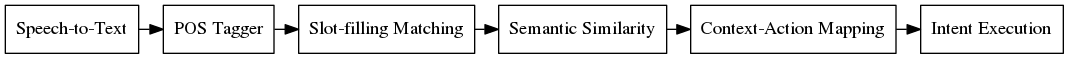
\includegraphics[width=\linewidth]{flow-chart.png}
  \caption{A flow chart showing the general stages of the voice recognition system. Graph generated using Graphviz.}
  \label{fig:flow-chart}
  \end{center}
\end{figure}
\end{center}

The steps are briefly described here and explained in more detail later on.

\begin{itemize}
\item The audio from the microphone input is processed into a text string using a Speech-to-Text (STT) engine. This string is then split up into a list of words.

\item The list of words is then used to generate a list of Part-of-Speech (POS) tags. Each word in the list is passed to the POS tagger and added to the tag list.

\item The word list is parsed using a slot-filling grammar, e.g. "\texttt{<ACTION> <TARGET> [with] <CONTEXT>}", or "\texttt{[use] <CONTEXT> [to] <ACTION> <TARGET>}".

\item When performing the matching, the current word being parsed is sent to a semantic similarity engine, and a similarity score is calculated.

\item If the player has specified an action to be done under a certain context, then the context-action mapping is consulted to find the correct method to execute. Otherwise, the default action method is chosen.

\item Finally, the in-game function is executed, and the text output is returned, with the game state updated.
\end{itemize}

\subsubsection{Speech-to-Text}

Android features a built-in speech recognition service, via its \texttt{SpeechRecognizer} class RRR, and this is used for the speech-to-text engine. While the API's primary method of speech recognition is via remote server communication, there is an option with the Android OS settings to perform offline speech recognition instead, by downloading the language data RRR.
\\
\\
Using this API, the player's utterance is transformed into a text string, which is then processed by the rest of the voice recognition system. Using an existing speech-to-text API means that less time is spent trying to get the player's utterance from the microphone input.
\\
\\
In terms of user interface, the application features an on-screen button containing the image of microphone. When the user presses this button, a voice request is initiated and lasts until the user finishes uttering their input. If the user doesn't say anything, then the response times out and is cancelled.

\subsubsection{POS Tagging}

For the Part-Of-Speech (POS) tagging of the input, the open-source Log-linear Part-Of-Speech Tagger provided by The Stanford Natural Language Processing Group will be used RRR. It is a Java archive file so can easily be imported and used in an Android Java project. It is a flexible API that handles all the POS tagging so no time needs to be spent implementing a POS tagging system. 
\\
\\
The software comes with two trained models. According to the software's \texttt{README} file, the first model uses a bidirectional architecture and includes training data using word shapes and distributional similarities. The second model uses a \textit{left3words} architecture, includes words shapes, and uses the Penn Treebank tagset. According to the developers, the bidirectional model is "slightly more accurate" with a correctness score of 97.28\%, but is much slower to tag with than the \textit{left3words} model. Therefore, the \textit{left3words} model was chosen to be used in the application. (It still features a performance correctness score of 96.97\% which is not that different to the bidirectional model's performance.)
\\
\\
With the input string broken down into an array list of its words, each word is used as input to the POS tagger, and the word's tag (e.g. \textit{VB}, \textit{NN}, etc.) is added to a new list. Both lists will be used simultaneously in other processes.

\subsubsection{Slot-filling Matching}

The next stage is to extract the important information from the input. In many applications, particularly in games, voice commands are usually given in the imperative form (such as, "do this", "attack that", etc.). We assume that the subject of the command (that is, the entity about whom the statement is made about RRR) is always the player (or the character that the player is controlling).
\\
\\
Generally, commands will have an imperative verb (e.g. "attack", "grab", "look"), optionally followed by the target entity for which the imperative verb should be applied towards, as well as an optional context entity for which the imperative verb should be applied with.
\\
\\
As an example, take the command, "hit the rock with a spoon". Here, the word 'hit' is the imperative action and it is applied to the 'rock'. The 'hit' action is applied using the 'spoon' as the context. The target and context help to provide a clearer intent; we could have just said, "hit" without mentioning the target or context, and while the action to be performed is clear, it is ambiguous as to what should be hit and with what.
\\
\\
For this stage, we use slot-filling structures (SFS) to describe the grammar of the voice commands. The SFS grammar chosen is as follows:

\begin{center}
\texttt{ACTION TARGET WITH CONTEXT}
\end{center}

Here, parts of the input will be mapped to a \textit{block} in the grammar. The \texttt{WITH} block represents words and phrases that signify using the context to perform the action (e.g. "with...", "using...", "with the power of the...", and so on). Figure \ref{fig:sfs-1} shows how parts of an example command are matched to the grammar.

\begin{center}
\begin{figure}[H]
\begin{center}
  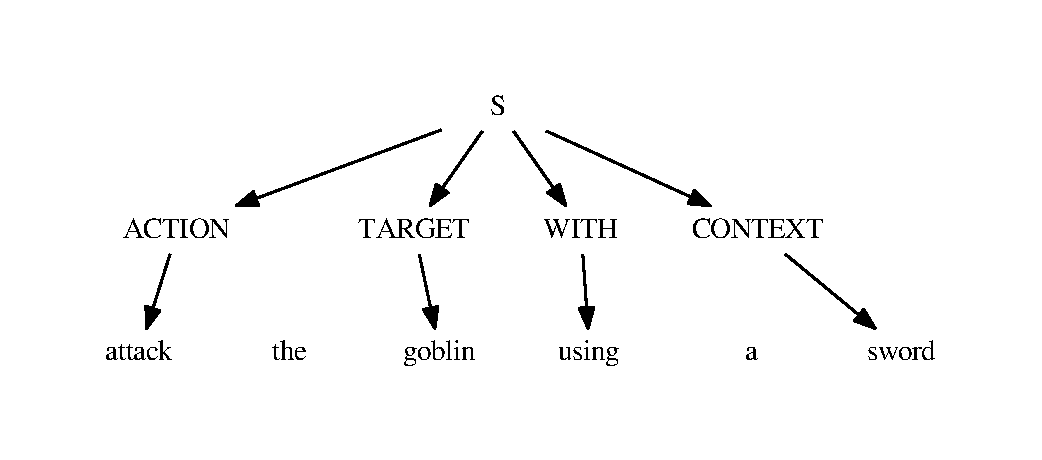
\includegraphics[width=\linewidth]{sfs-1.pdf}
  \caption{The slot-filling structure, \texttt{\{ACTION TARGET WITH CONTEXT\}} being applied to an example sentence, "attack the goblin using a sword". Generated using Graphviz.}
  \label{fig:sfs-1}
  \end{center}
\end{figure}
\end{center}

Not all the slots have to be filled; the \texttt{WITH} and \texttt{CONTEXT} blocks are completely optional to fill, but they provide more information about the user's intent. Should this information be left out, the system will fall back on the defaults for each one.
\\
\\
While this covers a large variety of commands that the user can give, such as, "attack the troll with a sword", "pick up the knife", or "look around the room using binoculars", it does not cover commands that have a completely different structure. For example, the phrases, "use a potion to heal" and "with a key open the door" are perfectly valid commands that a user can give, but the matching blocks are in completely different order (i.e. the \texttt{CONTEXT} comes before the \texttt{ACTION}), so would not be matched with the above SFS.
\\
\\
An alternative SFS is applied when appropriate. The grammar is as follows:

\begin{center}
\texttt{WITH CONTEXT ACTION TARGET}
\end{center}

Using this slot-filling grammar, the aforementioned example commands ("use a potion to heal" and "with a key open the door") would be accepted. Figure \ref{fig:sfs-2} shows an example of the matching.

\begin{center}
\begin{figure}[H]
\begin{center}
  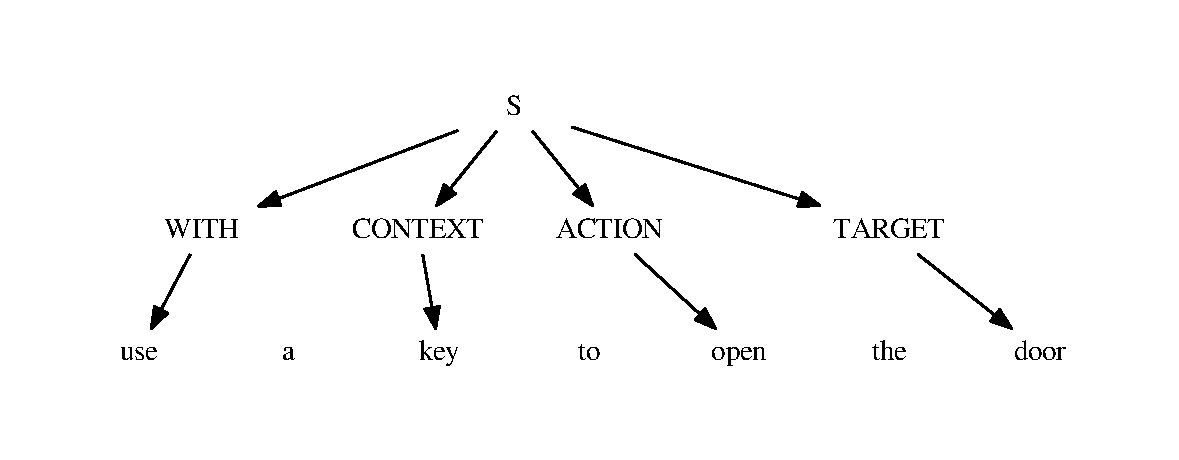
\includegraphics[width=\linewidth]{sfs-2.pdf}
  \caption{The slot-filling structure, \texttt{\{WITH CONTEXT ACTION TARGET\}} being applied to an example sentence, "use a key to open the door".}
  \label{fig:sfs-2}
  \end{center}
\end{figure}
\end{center}

During the processing, the correct SFS will be chosen based on the structure of the phrase (i.e. by determining the relative positions of each piece of information).
\\
\\
List of possible actions, targets and contexts are created by the developer (specified as strings), and the slot-filling matching will compare the words to the possible list of words to find a match.

\subsubsection{Semantic Similarity}

During the slot-filling  matching stage, if a word does not match any of the possible list of actions/targets/contexts character-by-character, then semantic similarity methods are used to determine the whether the two words are similar. For example, if the possible list of actions are, 'attack', 'heal' or 'run', and the input is 'hit', then 'hit' is more similar to the 'attack' action, so the 'attack' action would be chosen.
\\
\\
As mentioned before, there are many similarity methods that have been proposed. The first method to be used is the \textit{Wu and Palmer} method (WUP) described previously. Another method that is used is the \textit{Lin} method (LIN), that calculates the similarity of two words based on the information content of their lowest common subsumer (that is, their first common parent word in the WordNet hypernym tree) \cite{RefWorks:46}. Information content (IC) is defined as the negative log of the probability of a concept. The probability of a concept is based on the sense frequency of its synset.
\\
\\
Lin used IC to define a similarity measure similar to the Wu and Palmer method, but uses IC instead of the depths of the words in the word tree instead. The formula for the similarity of words $w_1$ and $w_2$ is as follows:

$$sim_{lin} = \frac{2*IC(LCS(w_1,w_2))}{IC(w_1)+IC(w_2)}$$

Another method used is the \textit{Lesk} method. The method determines the similarity of two words based on the overlaps in their definitions RRR. For instance, the definition for certain senses of the words, '\textit{ash}' and '\textit{coal}' (to describe a burnt substance) have the words, 'combustible', 'burn' and 'solid' in their definitions. Therefore, we can deduce that the words are semantically similar. In another paper, Banerjee and Pederson extended the Lesk method by using all the definitions of all the sense for both words in the calculation, as only using one sense definition did not give enough information RRR.
\\
\\
The WordNet database is accessed and traversed using the MIT Java WordNet Interface (JWI), which is an open-source library that interfaces with a WordNet database RRR. A full English WordNet database is downloaded from Princeton's website, and the JWI API is loaded with it.
\\
\\
Implementations for most of the similarity methods are provided by another open-source Java library, \textit{WS4J} RRR. While this library provides the methods for doing the calculations (such as the WUP, LIN and LESK formulas), the methods for the actual navigation and analysis of the WordNet database (e.g. getting hypernyms, synsets, glosses, etc.) must be implemented from scratch (see Implementation for details).

\subsubsection{Context-Action Mapping}

Once matches have been found from the slot-filling, they are mapped to the methods that should execute on that intent. If the player only specifies and action (and target) with no context, then a default action should be executed (the context itself defaults to a "default" context). If the player specifies a context (e.g. "...with a sword"), then a mapping is consulted to find the correct method that should be called. The different targets are handled within the method itself.
\\
\\
Table \ref{action-context-ex-table} shows an example of what an Context-Action map would look like. Note the \textit{null} entries that indicate that the context is not compatible with the corresponding action (for example, it does not make sense from a player to "attack with a potion"), and the intent is therefore ignored.

\begin{table}[H]
\centering
\caption{An example of an developer-specified Action-Context Mapping}
\label{action-context-ex-table}
\begin{tabular}{l|l|l|l|}
\cline{2-4}
\multicolumn{1}{c|}{\textbf{}}         & \multicolumn{3}{l|}{\textbf{actions}}                  \\ \hline
\multicolumn{1}{|l|}{\textbf{context}} & \textit{attack}    & \textit{heal}  & \textit{open}    \\ \hline
\multicolumn{1}{|l|}{\textit{default}} & AttackDefault()    & HealDefault()  & OpenDefault()    \\ \hline
\multicolumn{1}{|l|}{\textit{weapon}}  & AttackWithWeapon() & null           & OpenWithWeapon() \\ \hline
\multicolumn{1}{|l|}{\textit{potion}}  & null               & HealWithPotion & null             \\ \hline
\multicolumn{1}{|l|}{\textit{key}}     & AttackWithKey()    & null           & OpenWithKey()   \\ \hline
\end{tabular}
\end{table}

\subsubsection{Intent Execution}

Each non-null field in the Context-Action map contains a class that extends from an abstract class, \texttt{Action}. This abstract class contains an method called \texttt{run()}, which executes the in-game intent. This method is overridden by the derived classed (such as \texttt{AttackDefault} and \texttt{HealWithPotion}). These \texttt{run()} methods act as wrappers for the actual methods that would execute in the game (or to execute some other actions unrelated to the game, such as displaying the available commands, etc.)

\subsection{System UML Class Diagram}

Figure \ref{fig:system-overview} shows a simplified UML class diagram focusing on the classes used for the voice recognition system, including the inheritance and associations of the classes. Although the \texttt{GameState} class is related to the game system, it helps to illustrate the overall system design. Only the important member fields and methods are shown for each class.
\\
\\
See the Appendix \ref{appendix:system-uml} for the full UML class diagram of the Android application.

\begin{center}
\begin{figure}[H]
\begin{center}
  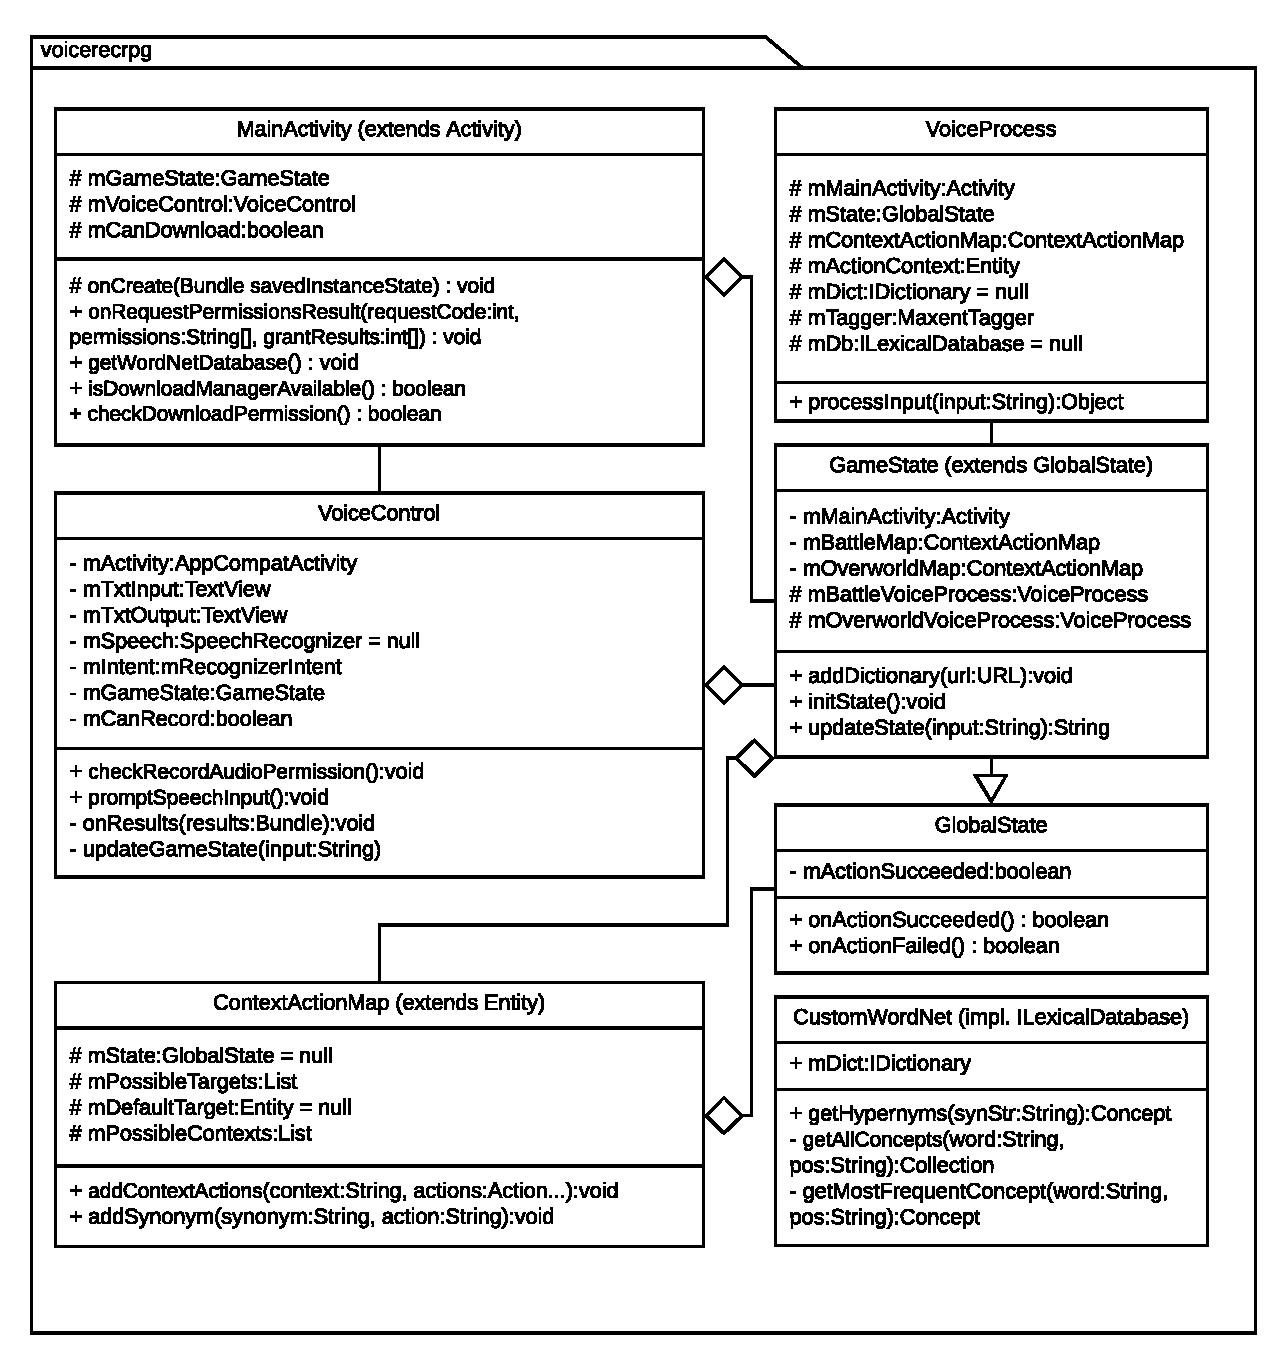
\includegraphics[width=\linewidth]{system-overview.pdf}
  \caption{A simplified UML class diagram outlining the design of the voice recognition system. Diagram created using the online LucidChart tool. See the Appendix \ref{appendix:game-uml} for the full class diagram for the entire voice recognition system in the Android application.}
  \label{fig:system-overview}
  \end{center}
\end{figure}
\end{center}

\subsubsection{\texttt{MainActivity} Class}

The \texttt{MainActivity} class is the skeleton class which contains all the systems. It acts as the interface between the I/O and the rest of the application. It contains instances of the \texttt{VoiceControl} class, which handles the I/O, and the \texttt{GameState}, which contains the game environment.
\\
\\
When the application starts up, an instance of \texttt{MainActivity} is created, and searches the public directory of the phone's external storage (not necessarily an external device like an SD card, but whatever the OS has has defined the external storage to be). It searches for a WordNet database that is downloaded beforehand, and if it is not found, it will download/re-download the database again. It will also copy a model used for POS tagging to the external storage from the APK archive.

\subsubsection{\texttt{VoiceControl} Class}

As mentioned, the \texttt{VoiceControl} class is used to handle the input and output of the application, such as the microphone input and the text display. It contains an instance of the SpeechRecognizer class, which is provided by Android and uses Google's Speech-to-Text API, as well as two instances of the TextView class: one which is used to display the text output of the game, and the other to display the Speech-to-Text result at the top of the screen.
\\
\\
When the \texttt{SpeechRecognizer} instance performs a Speech-to-Text translation, the final result is forwarded to the \texttt{GameState} instance where it is processed by the voice recognition system using NLP, and used to update the state of the current game session (\texttt{GameState}).

\subsubsection{\texttt{VoiceProcess} Class}

The \texttt{VoiceProcess} class is responsible for processing the string input containing the player's utterance that is received from the \texttt{VoiceControl} class. It contains the bulk of the NLP processing described later.

\subsubsection{\texttt{GlobalState} Class}

The \texttt{GlobalState} class is a generic abstract class that can be derived from in order to pass around environment objects between method calls easily. For example, if a method wishes to access an instance of an \texttt{Inventory} class (to access the game's items), then a reference to the inventory can be held in a class derived from \texttt{GlobalState} (e.g. \texttt{GameState}).

\subsubsection{\texttt{ContextActionMap} Class}

The \texttt{ContextActionMap} class contains the mapping of contexts to actions. It is an abstract class that is overloaded by the developer to add mappings of different ways of performing actions based on the given context (e.g. "attack with a sword" versus "attack with a knife").

\subsubsection{\texttt{SemanticSimilarity} Class}

This class contains the semantic similarity engine used for calculating the semantic similarity of two words as a confidence value between 0.0 and 1.0, based on information in the WordNet database. It uses a singleton design pattern so we don't have to instantiate the class every time we want to perform a calculation in a different method, nor do we have to pass a reference to an instance around. It also allows us to use the same static instance across different Android Activity contexts (and therefore allowing the engine's parameters to be changed in a \textit{Settings} activity).

\subsection{System Features}

In order to make the voice recognition system as as flexible as possible and able to infer the meanings of a wide variety for utterances, several mechanisms have been added to the system. These mechanisms help to reduce the amount of work required by the developer, and some are present in order to compensate for the shortcomings of the system (see the Evaluation section).

\subsubsection{Synonym Mapping}

The developer can map synonyms to actions if the words are not considered semantically similar by the system. For instance, if the word, "regenerate" has a low semantic similarity score when compared to the "heal" action, then the developer can create a map of "regenerate" $\rightarrow$ "heal" so the system performs the correct mapping.

\subsubsection{Ignoring Incorrect Matches}

Semantic similarity matches can be ignored if they are incorrectly mapped by the system, as a juxtaposition to the above feature.

\subsubsection{Confirmation and Suggestions}

If the user gives a command that has a confidence value just below the threshold, then the phrase is considered ambiguous and, using the possible candidate matches, suggestions are given to the user to confirm their intent. 
\\
\\
For example, if the user's intent is to pick up a knife and they say, "pick up the utensil", where the similarity score between "utensil" and "knife" is just below the threshold, the system will output, "Did you mean, 'pick up the knife? (yes/no)'", and waits for the user to respond. If they say no, then the system may suggest another alternative using the next ambiguous candidate (e.g, "Did you mean, 'pick up the plate?'", etc).

\subsubsection{Multiple Commands}

The user has the ability to execute a chain of several commands one after the other using just one utterance. For example, if the user says, "attack the enemy and then heal using a potion", this will execute two separate commands.

\subsubsection{Multiple Targets}

A user may want to execute a command that involves several targets. In this case, these are divided into several actions instead, with each action focused on one of the targets. For instance, if the user says, "attack the troll and the goblin", this will be split into two actions: one to attack the troll, followed by an attack on the goblin.

\subsubsection{Sentence Mapping}

The core mechanism of the system is the slot-filling structure described above. This covers most of the forms of possible imperative commands that a user may utter to the system to execute an intent. However, one disadvantage of this system is that it will not detect phrases that do not map to the slot-filling grammar given (e.g. \{\texttt{ACTION TARGET WITH CONTEXT}\}), despite being a valid phrase. Such utterances are usually phrased as a question, such as, "what actions can i do", or , "what items are in my bag", etc. We would like to still be able to detect these types of commands but prevent the user from hard-coding each possible variation of the intents.
\\
\\
The proposed solution is to perform sentence matching on these phrases. The developer specifies an intent followed by several example sentences that a user would say to execute the intent. For example, if the intent is to show the player the items they possess, example sentences include: "What is in my bag?", "What items do I have?", "What are the contents of my inventory?", and so on. When parsing a new utterance from the player (e.g. "what items are in my bag"), if the phrase fails the slot-filling stage, then the similarity of the sentence is calculated compared to the example sentences.
\\
\\
The calculation involves using a slightly altered cosine similarity method. Based on the formula for the cosine of an angle between two vectors, the cosine  similarity method measures uses the cosine of the angle as a measure of similarity, using a vector space model RRR (the vector of a sentence is represented by its word frequencies). The similarity between two vectors, $a$ and $b$ is:

$$similarity = \cos \theta = \frac{a \cdot b}{\lvert a\rvert\lvert b\rvert}$$

Take two examples: "the apples are in the tree" and "the tree contains apples". The vectors for these sentences would be:

\begin{center}
a = \{the:2, apples:1, are:1, in:1, the:2, tree:1, contains:0\}
\\
b = \{the:1, apples:1, are:0, in:0, the:1, tree:1, contains:1\}
\end{center}

The cosine similarity of these sentences is therefore:

$$\frac{a \cdot b}{\lvert a\rvert\lvert b\rvert} = \frac{6}{2\sqrt{3} \cdot \sqrt{5}} = 0.77$$

The definition for cosine similarity has been altered to form a "soft cosine measure" RRR. 
\\
\\
While the cosine similarity is not ideal for all situations (e.g. it ignores word order so may match two sentences which are not similar at all).

\subsection{Game Design Overview}

The voice recognition system will be applied to a text-based role-playing game that has several different modes of play, in order to demonstrate the flexibility of the system. The first mode is similar to the Zork-style text-adventure gameplay, mentioned previously. This involves the player interacting with objects in the environment to solve puzzles while collecting items, in order to progress. This mode is named the \textit{Overworld} mode
\\
\\
The second mode of gameplay is similar to classic turn-based RPGs such as Pokemon or Final Fantasy, where the player character battles an enemy, and the opposing sides alternate between taking turns to either attack, defend, heal, or perform some other action. This mode is called the \textit{Battle} mode.

\subsubsection{Game Flow}

The focus of the project is not on the game itself, but rather on the power and flexibility of the voice recognition system to add voice commands to the game itself. Therefore, only a very simple game will be created with only two rooms, with each room focusing on a different game mode (\textit{Overworld} or \textit{Battle}).
\\
\\
For the first room, the player is placed in a room where they are presented with a puzzle as part of the \textit{Overworld} mode. The room features the following description:

\begin{itemize}
\item "You are in a room with a locked door in front of you.

\item "There is a glass table in the middle of the room."

\item "There is a knife on the table."

\item "A painting of a tree hangs by a string on the left wall."
\end{itemize}

The player must obtain a key hidden behind the painting by cutting it down using the knife (or any other sharp item they may possess such as a sword), and then use the key to open the door.
\\
\\
During the overworld gameplay, the user is capable of performing the following actions:

\begin{center}
[look, show, grab, open, cut, break]
\end{center}

Example commands include, "show my inventory", "look around the room", "grab the knife", "cut the painting", and so on.
\\
\\
Each room in the game that features the overworld gameplay is represented by a finite state automaton. When the player performs certain actions (e.g. cutting the painting down), the state of the room will progress until the player has performed the correct  actions in the correct order and is able to progress to the next room. Figure \ref{fig:room1-fsa} show the state machine for the first room.

\begin{center}
\begin{figure}[H]
\begin{center}
  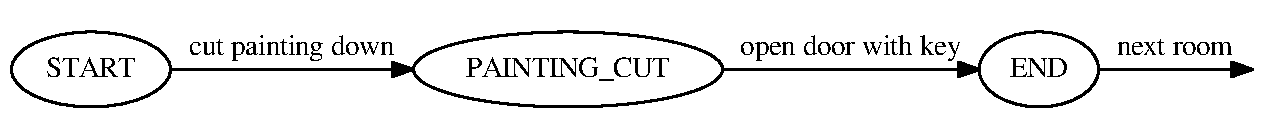
\includegraphics[width=\linewidth]{room1-fsa.pdf}
  \caption{The state machine for the first room in the game.}
  \label{fig:room1-fsa}
  \end{center}
\end{figure}
\end{center}

For the second room, the player is presented with a battle with an enemy (a \textit{troll}) as part of the \textit{Battle} mode.

\begin{center}
[attack, heal, show, look]
\end{center}

Examples include: "attack the troll" "heal with a potion", "look around", and so on.

\subsection{Game Design UML Class Diagram}

Figure \ref{fig:game-overview} shows a simplified UML class diagram for the game logic. See the Appendix for the full UML class diagram of the game logic.

\begin{center}
\begin{figure}[H]
\begin{center}
  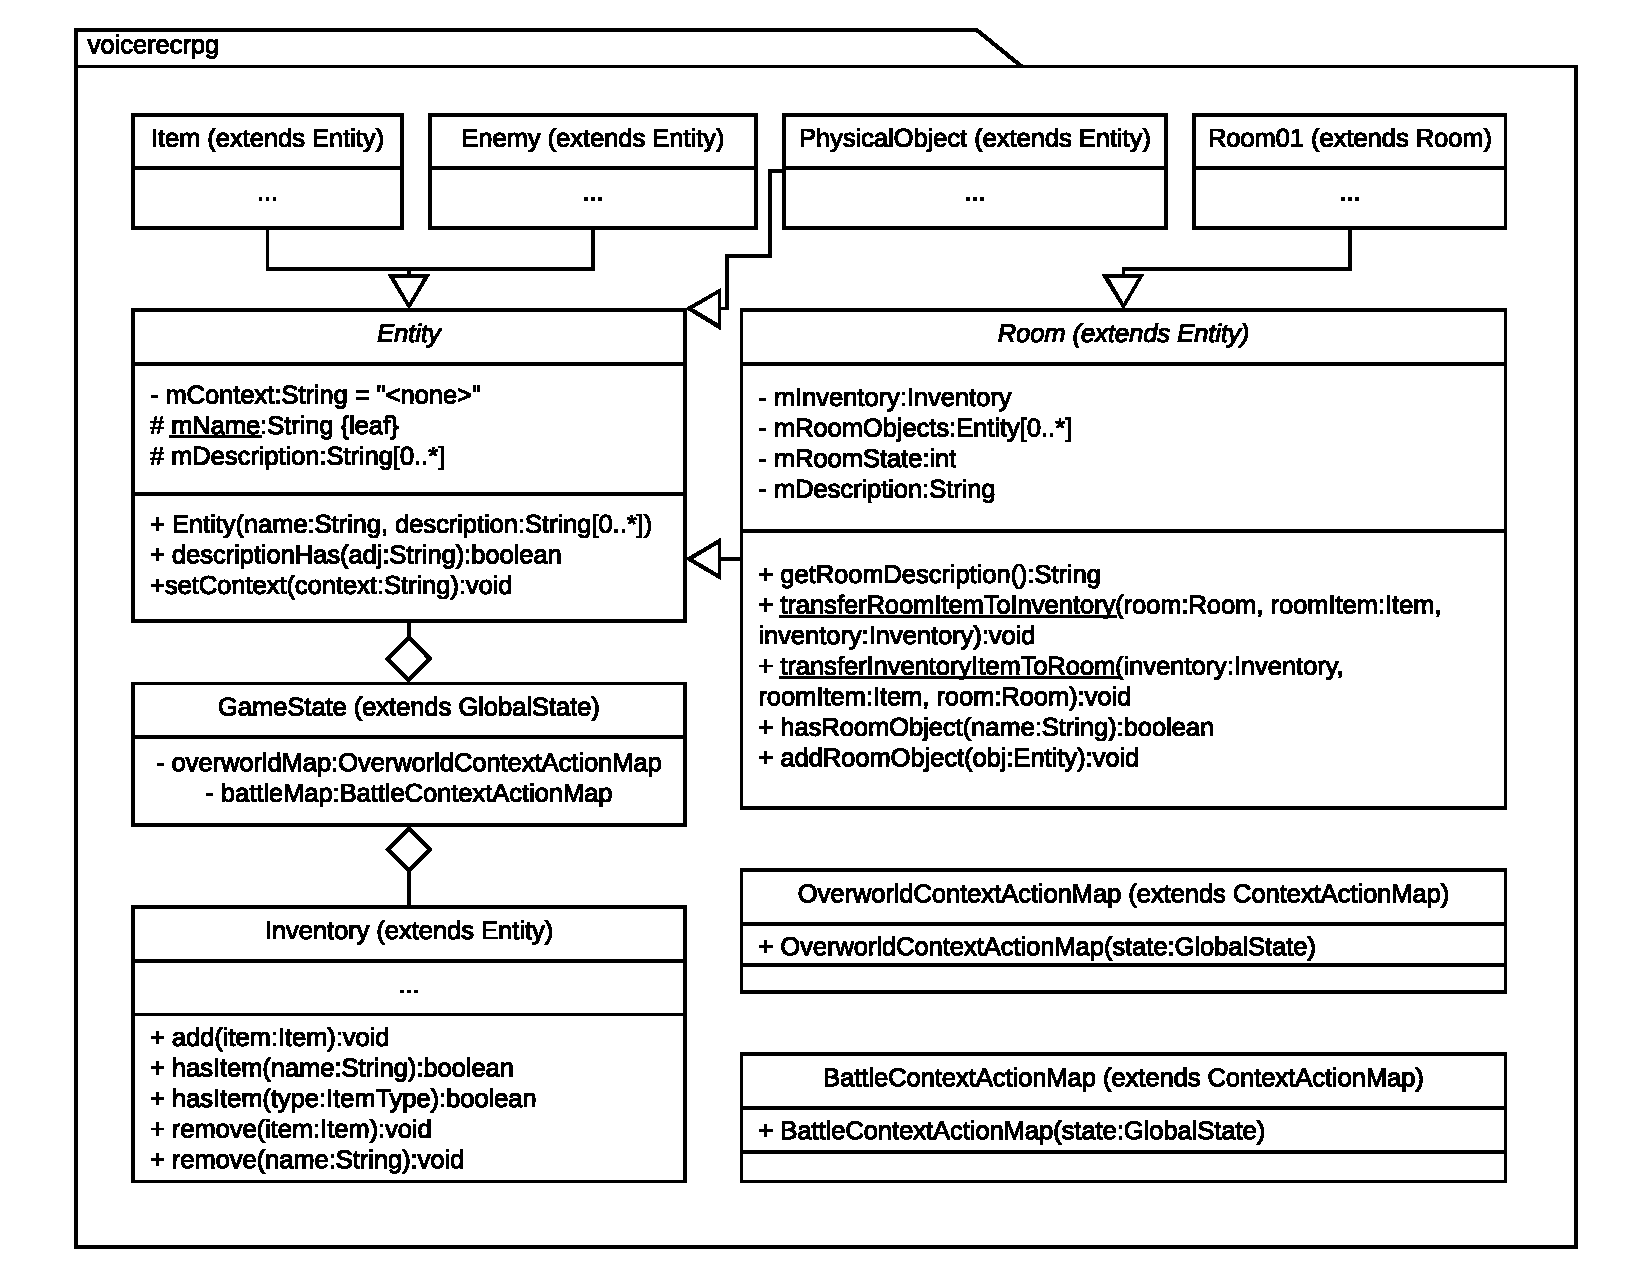
\includegraphics[width=\linewidth]{game-overview.pdf}
  \caption{A simplified UML class diagram outlining the design of the gameplay mechanics. Diagram created using the online LucidChart tool. See the Appendix for the full class diagram.}
  \label{fig:game-overview}
  \end{center}
\end{figure}
\end{center}

The \texttt{GameState} class (shown previously in the system UML class diagram, to aid explanations) contains two different instances of classes that override the voice recognition system's \texttt{ContextActionMap} class (which contain the voice command mappings): one for the overworld gameplay and the other for the battling gameplay.
\\
\\
The \texttt{Entity} abstract class represents anything that can be considered a possible target or context for the slot-filling. Each entity is given a name and a context type (as a string) that is used to determine which context it maps to (e.g. "weapon", "key", etc). See Table \ref{action-context-ex-table} above for examples of these contexts. Each entity also contains a description field which is an array of words that describe the entity (e.g. a knife would be described as "sharp", "pointy", etc). These descriptions are optional but they aid the voice recognition system to help identify similar words (if the semantic similarity match fails).
\\
\\
Finally, \texttt{Room} is an abstract class for generating new rooms for the game, each with their own objects.

\subsection{Room Generation}

Instead of forcing the developer to manually instantiate object within each room, a mechanism will be written that will allow a developer to generate a new room from just a description of it, using natural language processing techniques.

\newpage
\section{Implementation}

This section outlines the steps taken to implement the system and the game, mostly in chronological order where appropriate. For more details on the source code, please the corresponding GitHub repository containing this project's work.\footnote{https://github.com/BaronKhan/VoiceRecognitionRPG}

\subsection{Voice Recognition Interface}

The first step involved creating an Android project with a skeleton I/O to take as input the microphone audio, converts the speech to text, sends it to the voice recognition system for processing (initially just an empty class that pipes the input to output), before finally displaying the text on the screen.
\\
\\
The interface is within an Android \texttt{Activity} class. When the activity is created, it also downloads a tar ball containing a WordNet database and unzips it on the device's local storage. See the Appendix \ref{appendix:download} for a snippet of the code that downloads the database.
\\
\\
The \texttt{MainActivity} class contains a \texttt{VoiceControl} classes that  handles the speech-to-text (STT) I/O, and implements a \texttt{RecognizerIntent}. The \texttt{VoiceControl} object contains an instance of the \texttt{SpeechRecognizer} class that has a \texttt{startListening} method which invokes an \texttt{onResults()} method when finished. This method have a \texttt{results} parameter of type \texttt{Bundle}, containing the string result of the speech recognition. The string is then processed by an instance of the \texttt{VoiceProcess} class (described below).

\subsection{Graphical User Interface}

Figure \ref{fig:snapshot-ui} snapshot of the user interface for the game logic with the following labels:

\begin{enumerate}
	\item The player's input for the game as a string (i.e. it is the output of the speech-to-text API).
	\item The cumulative output as the game processes each user input.
	\item Pressing this button enables the microphone and starts a voice intent.
	\item A timer used for debugging the time taken to process an intent by the system.
	\item This drop-down list contains an option to open the settings menu.
\end{enumerate}

\begin{center}
\begin{figure}
\begin{center}
  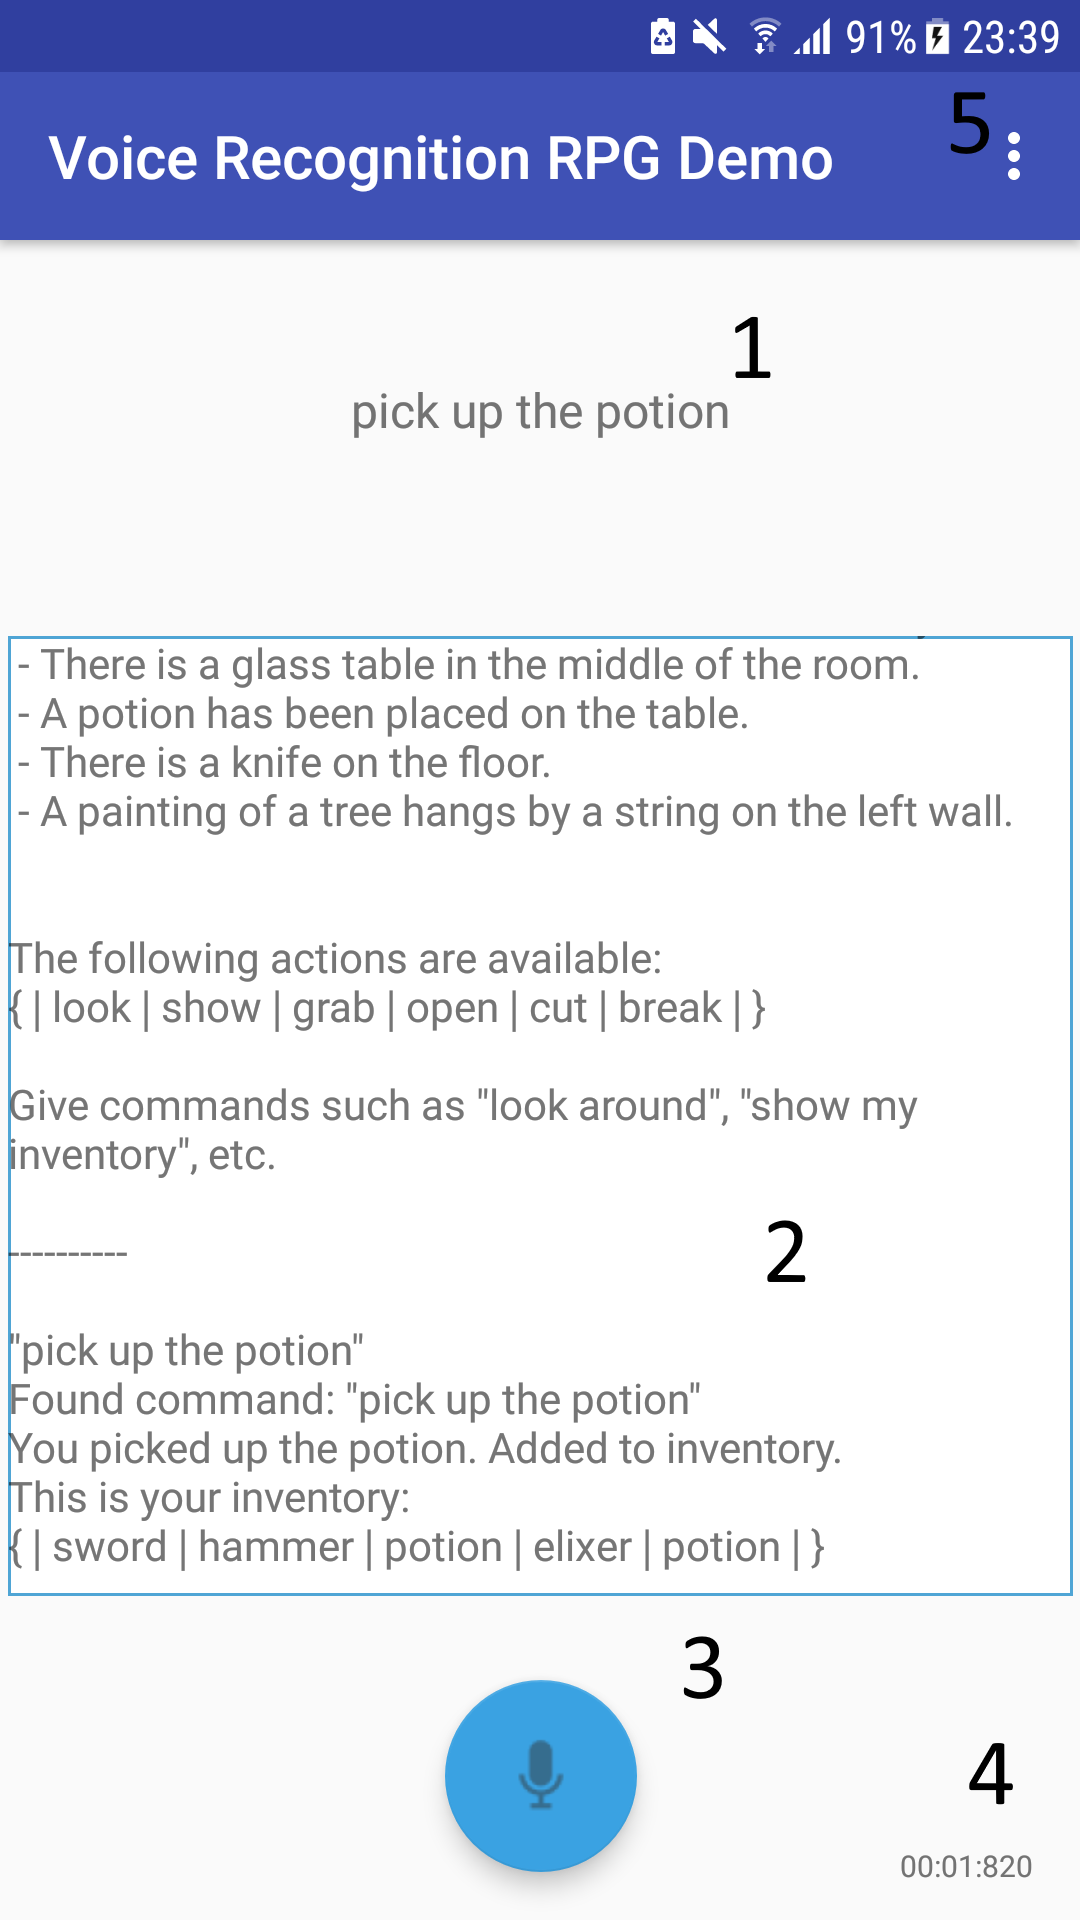
\includegraphics[scale=0.4]{Screenshot_20180519-233930.png}
  \caption{A snapshot of the user interface for the text-based role-playing game.}
  \label{fig:snapshot-ui}
  \end{center}
\end{figure}
\end{center}

All UI elements are accessed in the MainActivity and are separate from the voice recognition system.

\subsection{Voice Recognition System Implementation}

\subsubsection{GlobalState}

The \texttt{GlobalState} class is an abstract interface that sends the string input to a \texttt{VoiceProcess} instance via the \texttt{updateState} method. Derived classes (e.g. \texttt{GameState} for a game, \texttt{KitchenState} for a cooking application, etc.) contain the application-specific logic and environment that can be accessed by the action methods. Listing \ref{lst:global-state} shows the code for the \texttt{GlobalState} class.

\begin{lstlisting}[language=Java, caption=GlobalState.java, label={lst:global-state}]
package com.khan.baron.voicerecrpg.system;

//Derived classes should contain the environment objects to be used in actions
public abstract class GlobalState {
    protected boolean mActionSucceeded = true;
    
    public void actionSucceeded() { mActionSucceeded = true; }
    
    public void actionFailed() { mActionSucceeded = false; }
    
    public boolean getActionSucceeded() { return mActionSucceeded; }
    
    public abstract String updateState(String input);
}
\end{lstlisting}

In some scenarios, a follow-up action may only take place if the user's action was successful. For instance, in a generic two-player game, the second player may only be able to make their move once the first player has made a successful move. A more relevant example is in a turn-based role-playing game, where the player is fighting an enemy. The enemy can make their move once the player has made their move.
\\
\\
To support this scenario, there is a Boolean field called \texttt{mActionSucceeded}, which is set within the action methods that are executed to tell the system whether the action has succeeded, and the developer can choose what happens next.

\subsubsection{VoiceProcess.java}

\texttt{VoiceProcess.java} is the main class that performs all the processing on the text string input (of the user's utterance). The main method is the \texttt{processInput} method that takes the string input and returns the response. Listing \ref{lst:voice-process-pseudo} show the pseudocode for the method, with most of the details ignored (as it is a relatively long method). For the full Java method, refer to the source code in the project's repository.

\begin{lstlisting}[caption=VoiceProcess.processInput(), label={lst:voice-process-pseudo}]
def processInput(input):
    checkIfWordNetIsLoaded()
    
    if expectingReply:
        return processPendingIntent(input)
    
    //Check for action replies
    if currentAction.wantsReply():
        return currentAction.processReply(input)
    
    //Tokenise and tag the input
    words = input.split(" ")
    tags = getTags(words)
    if words.size() != tags.size:
        throw Exeception
    
    //Check for learning phrase ("___ means ___")
    if words.size() == 3 and words.contains("means"):
        addSynonym(words[0], words[2])
    
    //Parse the input
    actionIndex, chosenAction = getBestAction(words, tag)
    
    if isValidAction(actionStr):
        chosenTarget = getBestTarget(words, tags)
        chosenContext = getBestContext(words, tags)
        
        if not isValidContext(bestContext):
                or contextActionMap.get(chosenContext).get(chosenAction) == null:
            chosenContext = "default"
            
        action = contextActionMap.get(chosenContext).get(chosenAction)
        if action == null:
            return "Intent not understood."
        else:
            if isAmbiguous():
                return suggestion()	//Did you mean...?
            else:
                 return action.execute(state, chosenTarget)
    else:
    	//Check for another target for previous action
        if foundAnotherTarget(words, tags):
            currentTarget = getBestTarget(words, tags)
            return previousAction.execute(state, currentTarget)
        else if foundAnotherContext(words, tags):
            currentContext = getBestContext(words, tags)
            return previousAction.execute(state, currentContext)
        else:
            performSentenceMatching(input)
\end{lstlisting}

\subsubsection{SemanticSimilarity.java}

The semantic similarity engine uses a singleton design pattern so that it doesn't have to be constantly instantiated whenever a calculation is made. 




















\newpage
\section{Appendix}
\subsection{Skyrim Kinect Command List}
\label{appendix:skyrim}
Below is a list of all 200 commands that can be used in the video game, The Elder Scrolls V: Skyrim, when a Microsoft Kinect peripheral is connected.

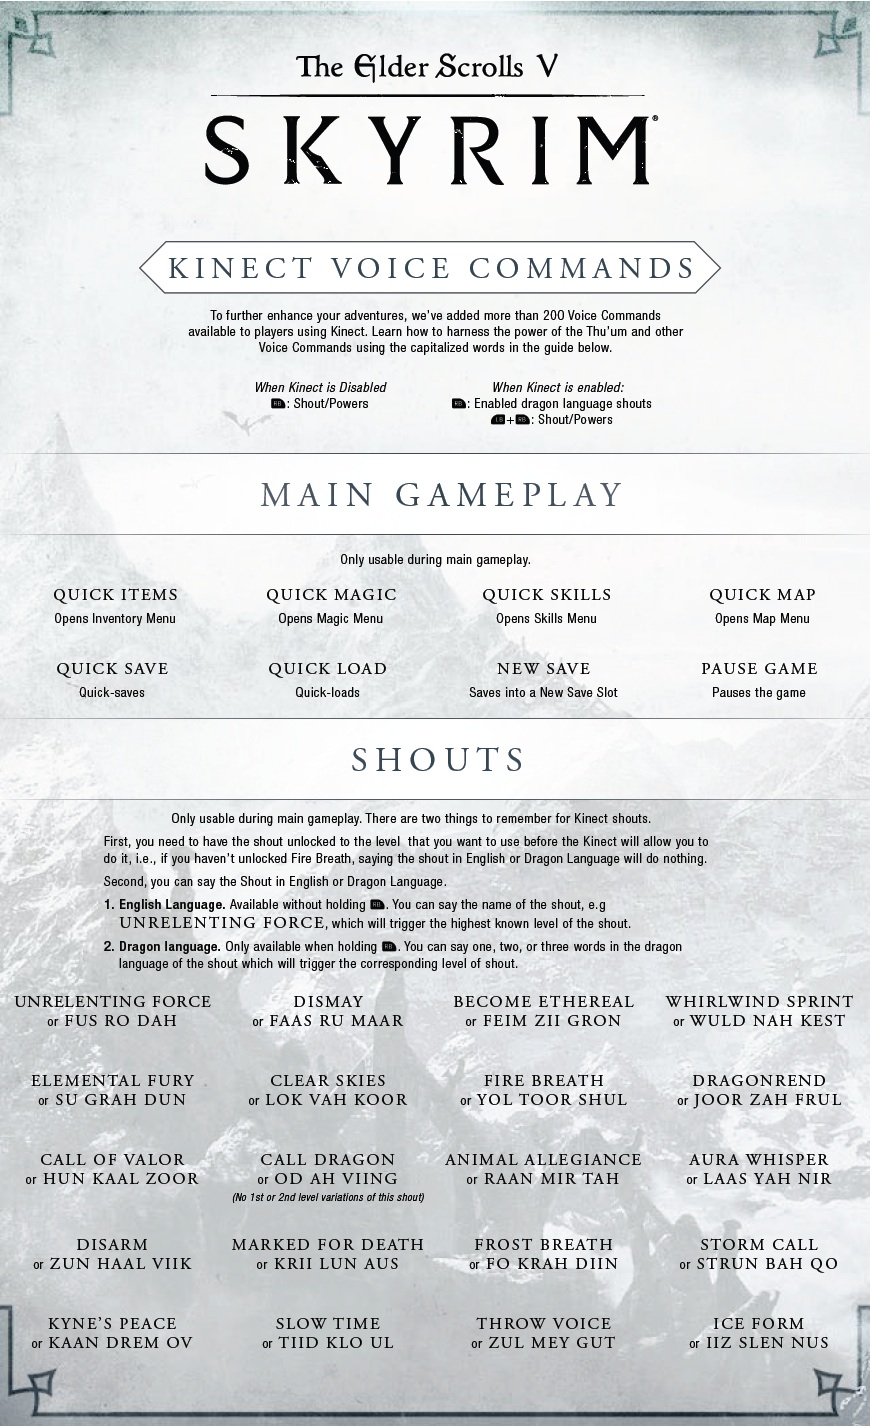
\includegraphics[scale=0.235]{skyrim-1.jpg}
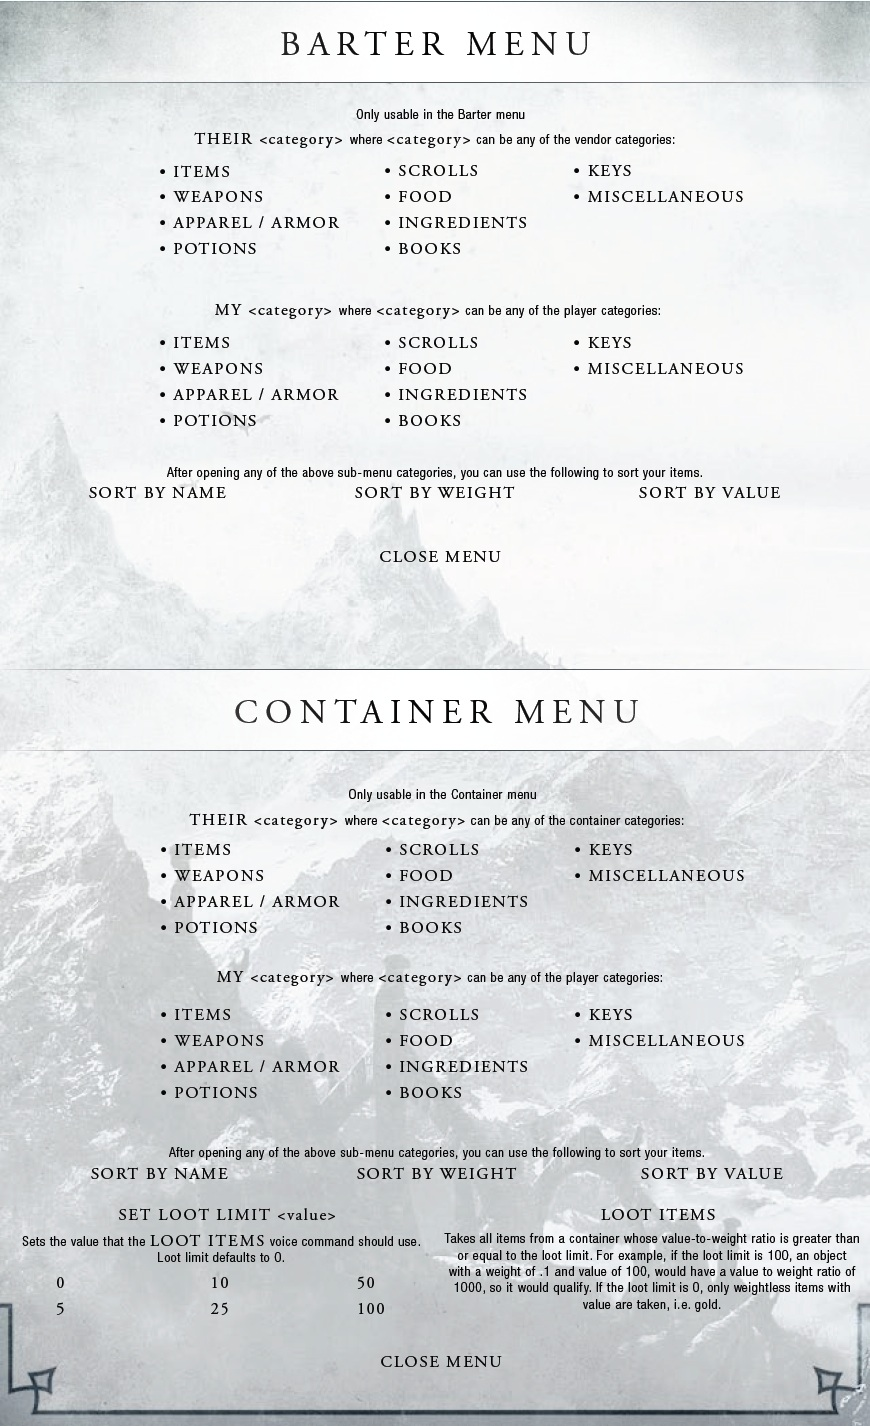
\includegraphics[scale=0.235]{skyrim-2.jpg}
\newpage
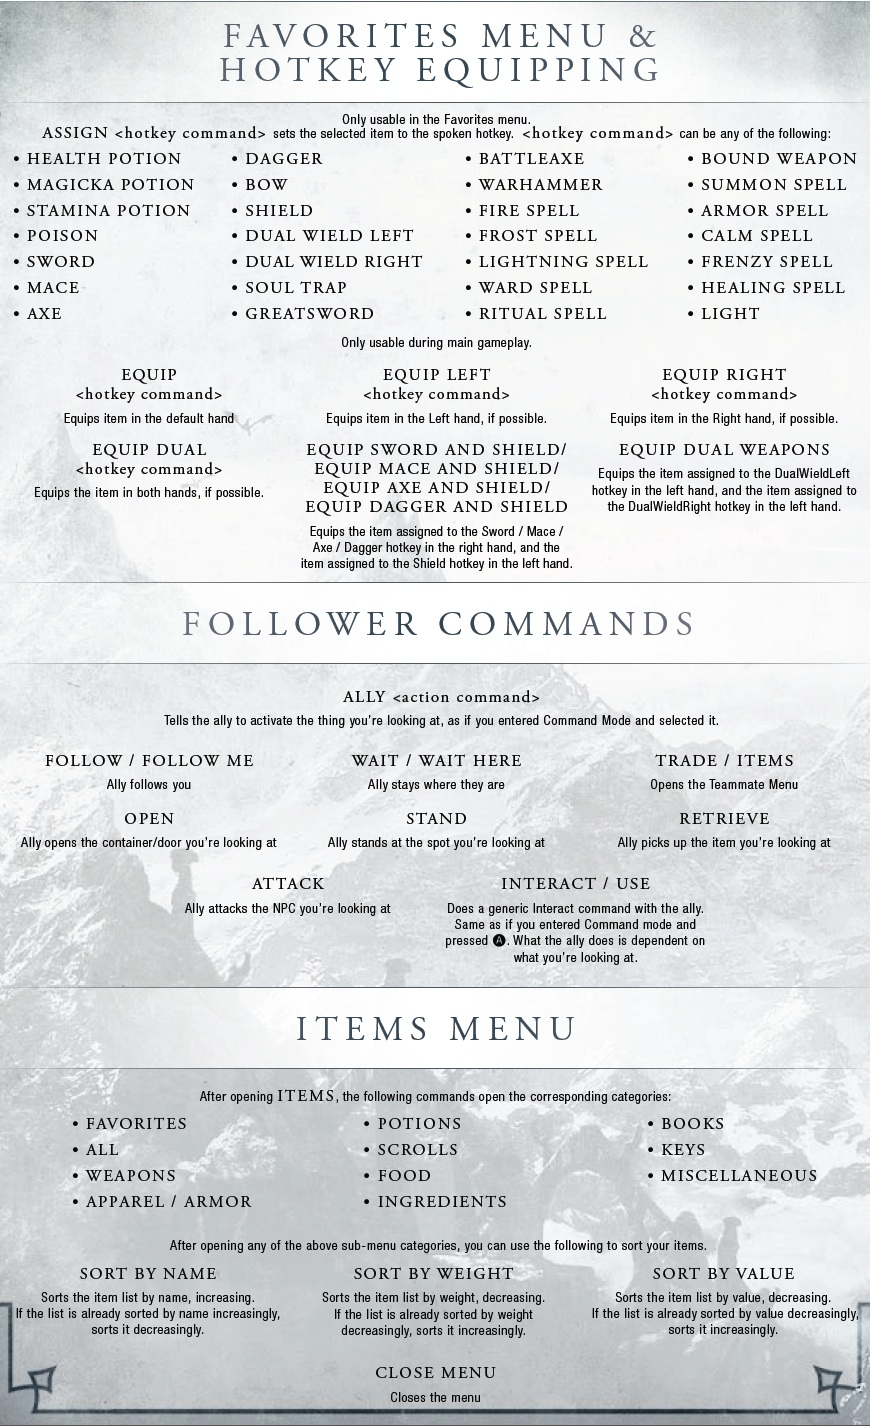
\includegraphics[scale=0.237]{skyrim-3.jpg}
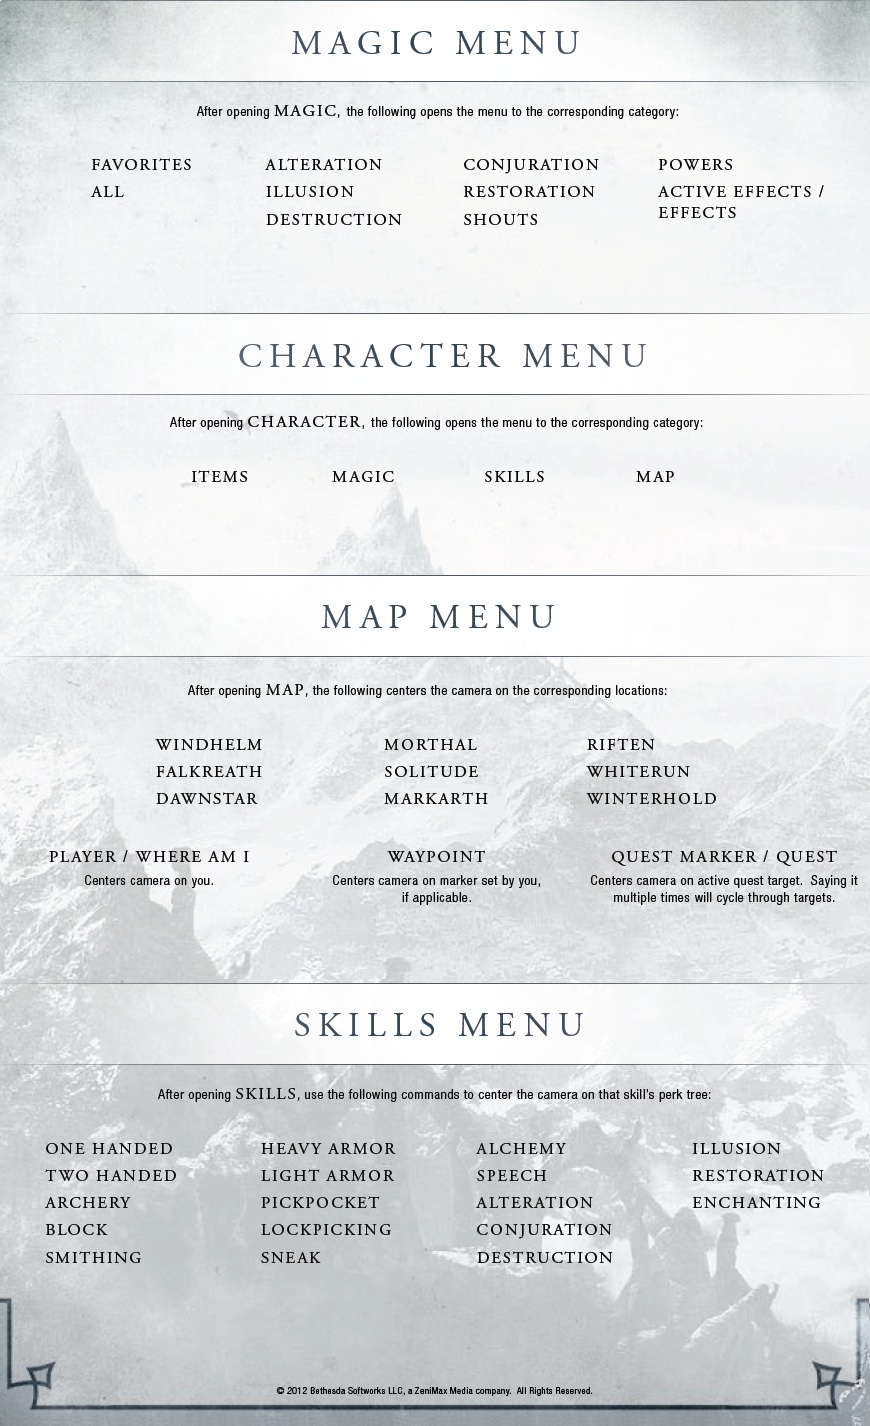
\includegraphics[scale=0.237]{skyrim-4.jpg}
\newpage
\subsection{Penn Treebank Tagset}
\label{appendix:penn}

Below is a table of the 32 tags from the Penn Treebank tagset, used for POS tagging. The 12 remaining tags for punctuation and other symbols have been left out \cite{RefWorks:42}.

$$
\begin{tabular}{ |p{3.25cm}|p{3.25cm}|p{3.25cm}|p{3.25cm}| }
\hline
	CC & Coordinating\ conjunction & TO & to \\ \hline
	CD & Cardinal\ number & UH & Interjection \\ \hline
	DT & Determiner & VB & Verb, base\ form \\ \hline
	EX & Existential\ there & VBD & Verb, past\ tense \\ \hline
	FW & Foreign\ word & VBG & Verb, gerund\ or\ present\ participle \\ \hline
	IN & Preposition\ or\ subordinating conjunction & VBN & Verb, past\ participle \\ \hline
	PRP\$ & Possessive\ pronoun & NNS & Noun,\ plural \\ \hline
	RB & Adverb & NNP & Proper\ noun,\ singular \\ \hline
	RBR & Adverb,\ comparative & NNPS & Proper\ noun, plural \\ \hline
	RBS & Adverb,\ superlative & PDT & Predeterminer \\ \hline
	RP & Particle & POS & Possessive\ ending \\ \hline
	SYM & Symbol & PRP & Personal\ pronoun \\ \hline
	JJ & Adjective & VBP & Verb, non-3rd\ person\ singular\ present \\ \hline
	JJR & Adjective, comparative & VBZ & Verb, 3rd\ person\ singular\ present \\ \hline
	JJS & Adjective,\ superlative & WDT & Wh-determiner \\ \hline
	LS & List\ item\ marker & WP & Wh-pronoun \\ \hline
	MD & Modal & WP\$ & Possessive\ wh-pronoun \\ \hline
	NN & Noun,\ singular\ or\ mass & WRB & Wh-adverb \\ \hline
\end{tabular}
$$

\newpage
\subsection{System UML Class Diagram}
\label{appendix:system-uml}
Below is the UML class diagram for the voice recognition system used in the Android app. This was automatically generated using the third-party \textit{simpleUML} plugin for Android Studio.
\\
\\
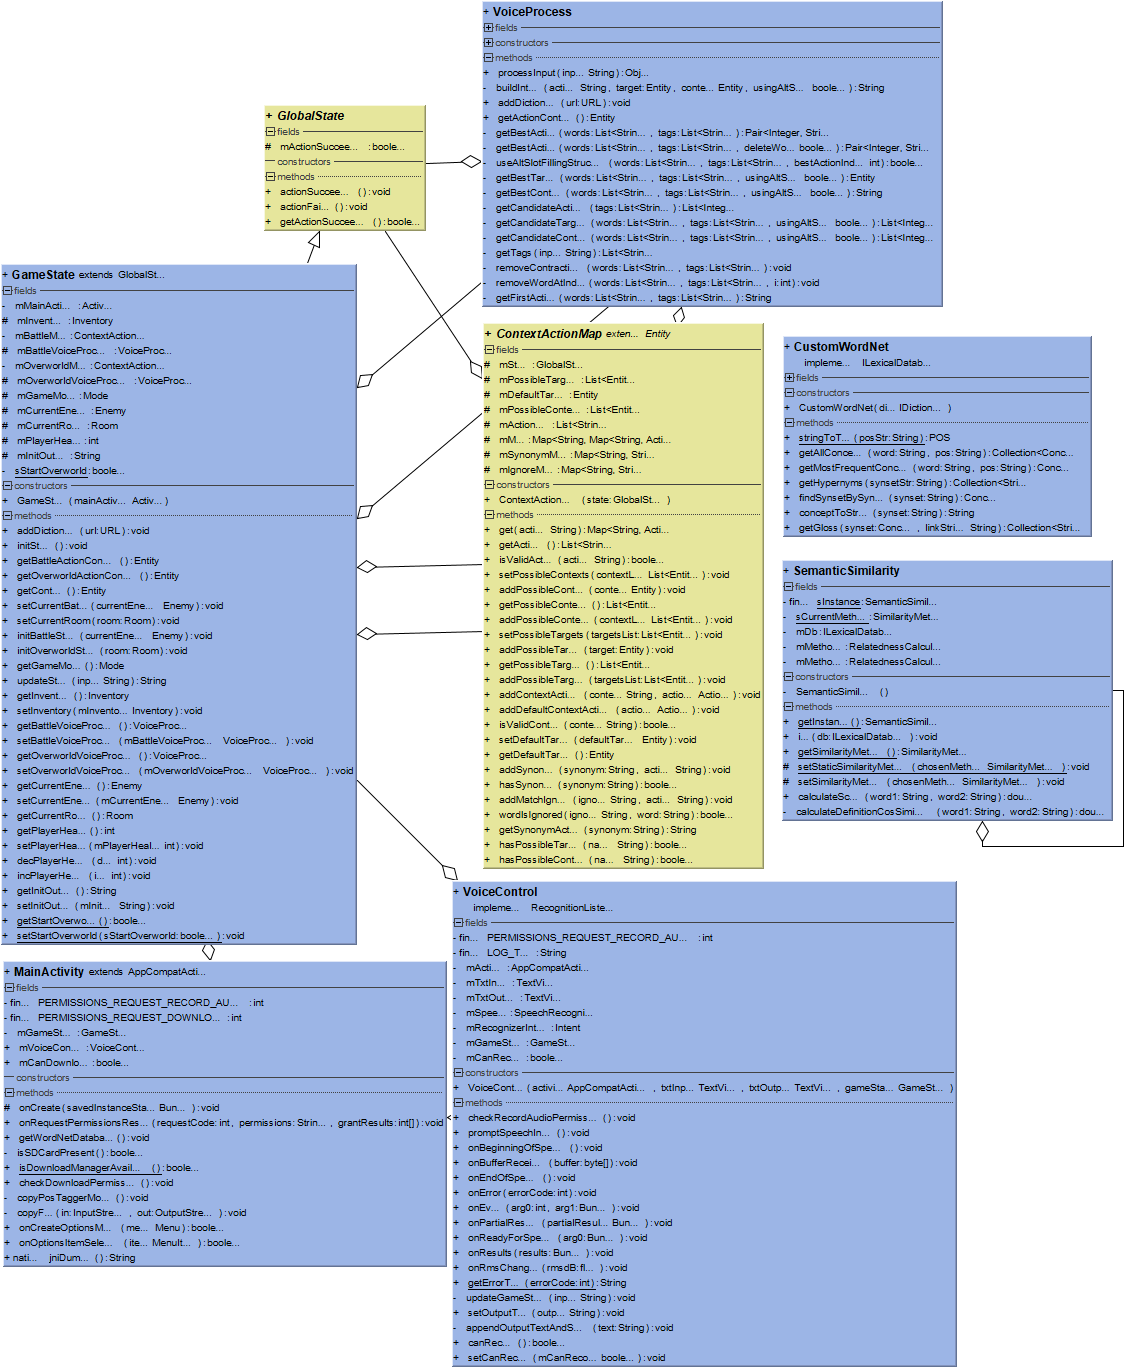
\includegraphics[scale=0.37]{system-uml.png}

\newpage
\subsection{Game Design UML Class Diagram}
\label{appendix:game-uml}
Below is the UML class diagram for the game mechanics - both the \textit{Overworld} and \textit{Battle} game modes. Generated using the third-party \textit{simpleUML} Android plugin.
\\
\\
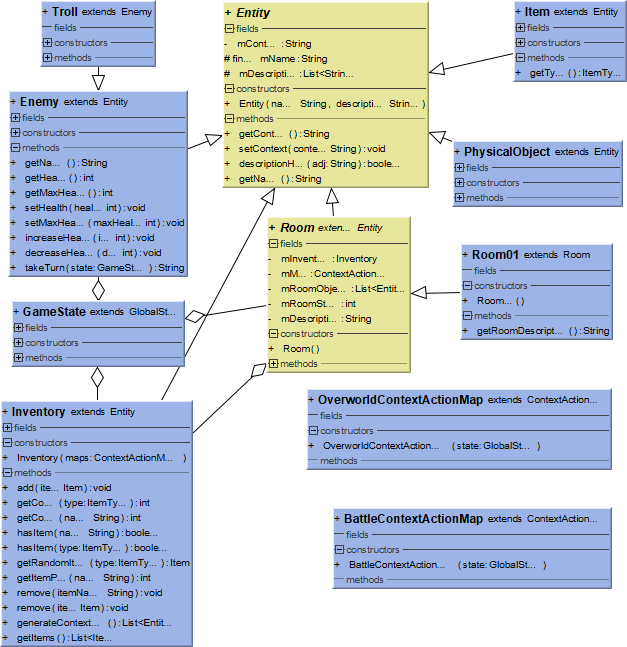
\includegraphics[width=\textwidth]{game-uml.png}

\newpage
\subsection{WordNet Download Code}
\label{appendix:download}
\begin{lstlisting}[language=Java, caption=MainActivity.getWordNetDatabase()]
public void getWordNetDatabase() throws IOException {
    boolean foundWordNetDatabase = false;
    if (!isSDCardPresent()) {
        Snackbar.make(findViewById(R.id.activity_main),
                "Error: SD card not mounted. Cannot access WordNet database.",
                Snackbar.LENGTH_LONG).setAction("Action", null).show();
        return;
    }

    File dictFile = new File(Environment.getExternalStorageDirectory().getPath()+"/dict/");
    if(dictFile.exists()) {
        Snackbar.make(findViewById(R.id.activity_main), "Found WordNet database",
                Snackbar.LENGTH_LONG).setAction("Action", null).show();
        foundWordNetDatabase = true;

    } else {
        if (isDownloadManagerAvailable()) {
            Snackbar.make(findViewById(R.id.activity_main), "Downloading WordNet database...",
                    Snackbar.LENGTH_LONG).setAction("Action", null).show();

            checkDownloadPermission();
            if (!mCanDownload) {
                Snackbar.make(findViewById(R.id.activity_main),
                        "Error: permission not given to download WordNet database",
                        Snackbar.LENGTH_LONG).setAction("Action", null).show();
                return;
            }

            File archive = new File(
                    Environment.getExternalStoragePublicDirectory(
                            Environment.DIRECTORY_DOWNLOADS) + "/wn3.1.dict.tar.gz");
            if(!archive.exists()) {
                String url = "http://wordnetcode.princeton.edu/wn3.1.dict.tar.gz";
                DownloadManager.Request request = new DownloadManager.Request(Uri.parse(url));
                request.setDescription("Downloading WordNet database...");
                request.setTitle("WordNet Database");
                if (Build.VERSION.SDK_INT >= Build.VERSION_CODES.HONEYCOMB) {
                    request.allowScanningByMediaScanner();
                    request.setNotificationVisibility(
                            DownloadManager.Request.VISIBILITY_VISIBLE_NOTIFY_COMPLETED);
                }
                request.setDestinationInExternalPublicDir(
                        Environment.DIRECTORY_DOWNLOADS, "wn3.1.dict.tar.gz");
                DownloadManager manager = (DownloadManager) getSystemService(
                        Context.DOWNLOAD_SERVICE);
                manager.enqueue(request);
                BroadcastReceiver onComplete=new BroadcastReceiver() {
                    public void onReceive(Context ctxt, Intent intent) {
                        try {
                            getWordNetDatabase();
                        } catch (Exception e) {
                            mVoiceControl.setOutputText("Error: " + e.getMessage());
                        }
                    }
                };
                registerReceiver(onComplete, new IntentFilter(
                        DownloadManager.ACTION_DOWNLOAD_COMPLETE));
            } else {

                // Extract tarball
                File dest = new File(Environment.getExternalStorageDirectory().getPath());
                TarArchiveInputStream fin = new TarArchiveInputStream(
                        new GzipCompressorInputStream(new FileInputStream(archive.getPath())));
                TarArchiveEntry entry;
                while ((entry = fin.getNextTarEntry()) != null) {
                    if (entry.isDirectory()) {
                        continue;
                    }
                    File curfile = new File(dest, entry.getName());
                    File parent = curfile.getParentFile();
                    if (!parent.exists()) {
                        parent.mkdirs();
                    }
                    IOUtils.copy(fin, new FileOutputStream(curfile));
                }

                Snackbar.make(findViewById(R.id.activity_main), "Downloaded WordNet database",
                        Snackbar.LENGTH_LONG).setAction("Action", null).show();

                foundWordNetDatabase = true;
            }

        } else {
            Snackbar.make(findViewById(R.id.activity_main),
                    "Error: could not download WordNet database", Snackbar.LENGTH_LONG)
                    .setAction("Action", null).show();
            return;
        }
    }
}
\end{lstlisting}

\newpage
\addcontentsline{toc}{section}{References}
\bibliography{references}
\end{document}
